\chapter{Implemetasi Website BlueTape dengan Bootstrap 4}
Bab 4 menjelaskan implementasi untuk mengubah seluruh tampilan website dengan framework Bootstrap 4 pada website BlueTape.
\section{Konversi Tampilan dengan Bootstrap 4}
Pada bagian ini akan dijabarkan keseluruhan kelas yang dipakai dalam website BlueTape. Pertama akan dijabarkan file framework yang digunakan, kemudian akan dijelaskan komponen yang digunakan dalam website BluTape dan terakhir penggunaan kelas framework Bootstrap 4 pada website.
\subsection{Menjalankan Framework Bootstrap 4}
Website BlueTape menggunakan sebuah framework PHP yaitu CodeIgniter. Hal pertama yang dilakukan saat ingin menjalankan tampilan adalah cek terlebih dimana file yang berkaitan dengan Framework Bootstrap 4 disimpan, lalu dilihat file tersebut dijalankan ketika membangun sebuah tampilan. 
\subsection{Folder untuk Menyimpan File Bootstrap 4 dan Plugin}
Seluruh file terkait dengan Framework Bootstrap 4 diletakkan dalam folder \texttt{/www/public}. Dimana terdiri dari folder:
%direferensikan di bab2
\begin{enumerate}
	\item css: Terdiri dari file - file css dari beserta file ikon bawaan dari framework Bootstrap 4. 
	\item img: Menyimpan sebuah gambar logo BlueTape. 
	\item js: Menyimpan file javascript bawaan dari Bootstrap 4 dan file jquery yang tersimpan dalam folder vendor.
	\item lib: Menyimpan plugin xdan-datetimepicker.
\end{enumerate}


\subsection{Folder untuk Implementasi Framework Bootstrap 4 dan Plugin}
Untuk melihat code tampilan website, maka \textit{user} akan mengakses file - file dalam folder \texttt{/www/application/views/}. Folder views terdiri dari beberapa sub-folder. Secara garis besar, file terdiri dari dua fungsi yaitu menyimpan kode template yang digunakan untuk keseluruhan tampilan dan implementasi komponen - komponen Bootstrap 4 untuk membangun sebuah website. \\

Pertama untuk sub-folder template terdiri dari: 
\begin{enumerate}
	\item auth	: Berisi file terkait dengan framework Bootstrap 4 akan diimport disini, kemudian akan disertakan sebuah tampilan login dan notifikasi - notifikasi terkait dengan status login. File tersebut tercatat di \texttt{login.php}.
	\item error	: Berisi folder untuk mengatasi error ketika user gagal untuk \textit{load} tampilan. Pesan akan ditampilkan pada \textit{user} ketika error terjadi. Folder ini sudah ada sejak pertama mengunduh framework CodeIgniter.
	\item templates	: Folder ini mencangkup kode template yang digunakan untuk seluruh bagian website BlueTape. 
%	Terdiri dari:
%	\begin{itemize}
%		\item flashmessage Menyimpan notifikasi terkait dengan autentikasi ketika login ke dalam website.
%		\item head$\_$loggedin Another descriptive item
%		\item script$\_$Bootstrap 4 And another descriptive item
%		\item head$\_$loggedin And another descriptive item
%	\end{itemize}
\end{enumerate}

Lalu sub-folder template yang berfungsi untuk menyimpan kode tampilan website terdiri 6 folder. Masing - masing folder memiliki sebuah file \texttt{main.php}. Sub-folder tersebut yaitu:
\begin{enumerate}
	\item EntriJadwalDosen
	\item LihatJadwalDisen
	\item PerubahanKuliahManage
	\item PerubahanKuliahRequest
	\item TranskripManage
	\item TranskripRequest
\end{enumerate}

\subsection{Import File Bootstrap 4}
File \texttt{head$\_$loggedin.php} akan memanggil semua file css terkait dengan file Bootstrap 4.
\begin{lstlisting}[frame=single, basicstyle=\small]
<?php
defined('BASEPATH') OR exit('No direct script access allowed');
?><head>
<meta charset="utf-8" />
<meta http-equiv="x-ua-compatible" content="ie=edge">
<meta name="viewport" content="width=device-width, initial-scale=1.0" />
<title><?= $this->config->item('module-names')[$currentModule] ?></title>
<link rel="stylesheet" href="/public/css/bootstrap.css" />
<link rel="stylesheet" href="/public/css/app.css" />
<link rel="stylesheet" href="/public/lib/xdan-datetimepicker/
jquery.datetimepicker.min.css" />
</head>.
\end{lstlisting}
Kemudian untuk file jquery dan javascript yang digunakan dalam Bootstrap 4 akan dipanggil dalam file script$\_$Bootstrap 4.php
\begin{lstlisting}[frame=single, basicstyle=\small]
<?php
defined('BASEPATH') OR exit('No direct script access allowed');
?>
<script src="/public/js/vendor/jquery.min.js"></script>
<script src="/public/js/vendor/what-input.min.js"></script>
<script src="/public/js/Bootstrap 4.min.js"></script>
<script src="/public/js/app.js"></script>
<script src="/public/lib/xdan-datetimepicker/
jquery.datetimepicker.full.min.js"></script>
\end{lstlisting}

\subsection{Grid System Bootstrap 4 dalam Website BlueTape}
Keseluruhan tampilan pada website menggunakan kelas \texttt{float grid} dimana sebelum menggunakan komponen, elemen akan mengimplementasikan kelas:
\begin{itemize}
	\item \texttt{.container}: Halaman website BlueTape yang memiliki satu konten akan diletakkan dalam kelas ini.
	\begin{itemize}
		\item Halaman Transkrip Manage
		\item Halaman Perubahan Kuliah Manage
	\end{itemize}
	%Buat analisis khusus kelas .row	
	\item \texttt{.container column}: Untuk halaman yang memiliki lebih dari satu konten akan dimasukan dalam kombinasi kelas dari \texttt{.row} dan \texttt{.column} sehingga konten berbaris secara vertikal.  Halaman yang menggunakan kelas ini adalah:
	\begin{itemize}
		\item Halaman Perubahan Kuliah Request
		\item Halaman Transkrip Request
		\item Halaman Lihat Jadwal Dosen
		\item Halaman Entri Jadwal Dosen
	\end{itemize}	
	
\end{itemize}

\subsection{Navigation Bar}
\begin{figure} [H]
	\centering  
	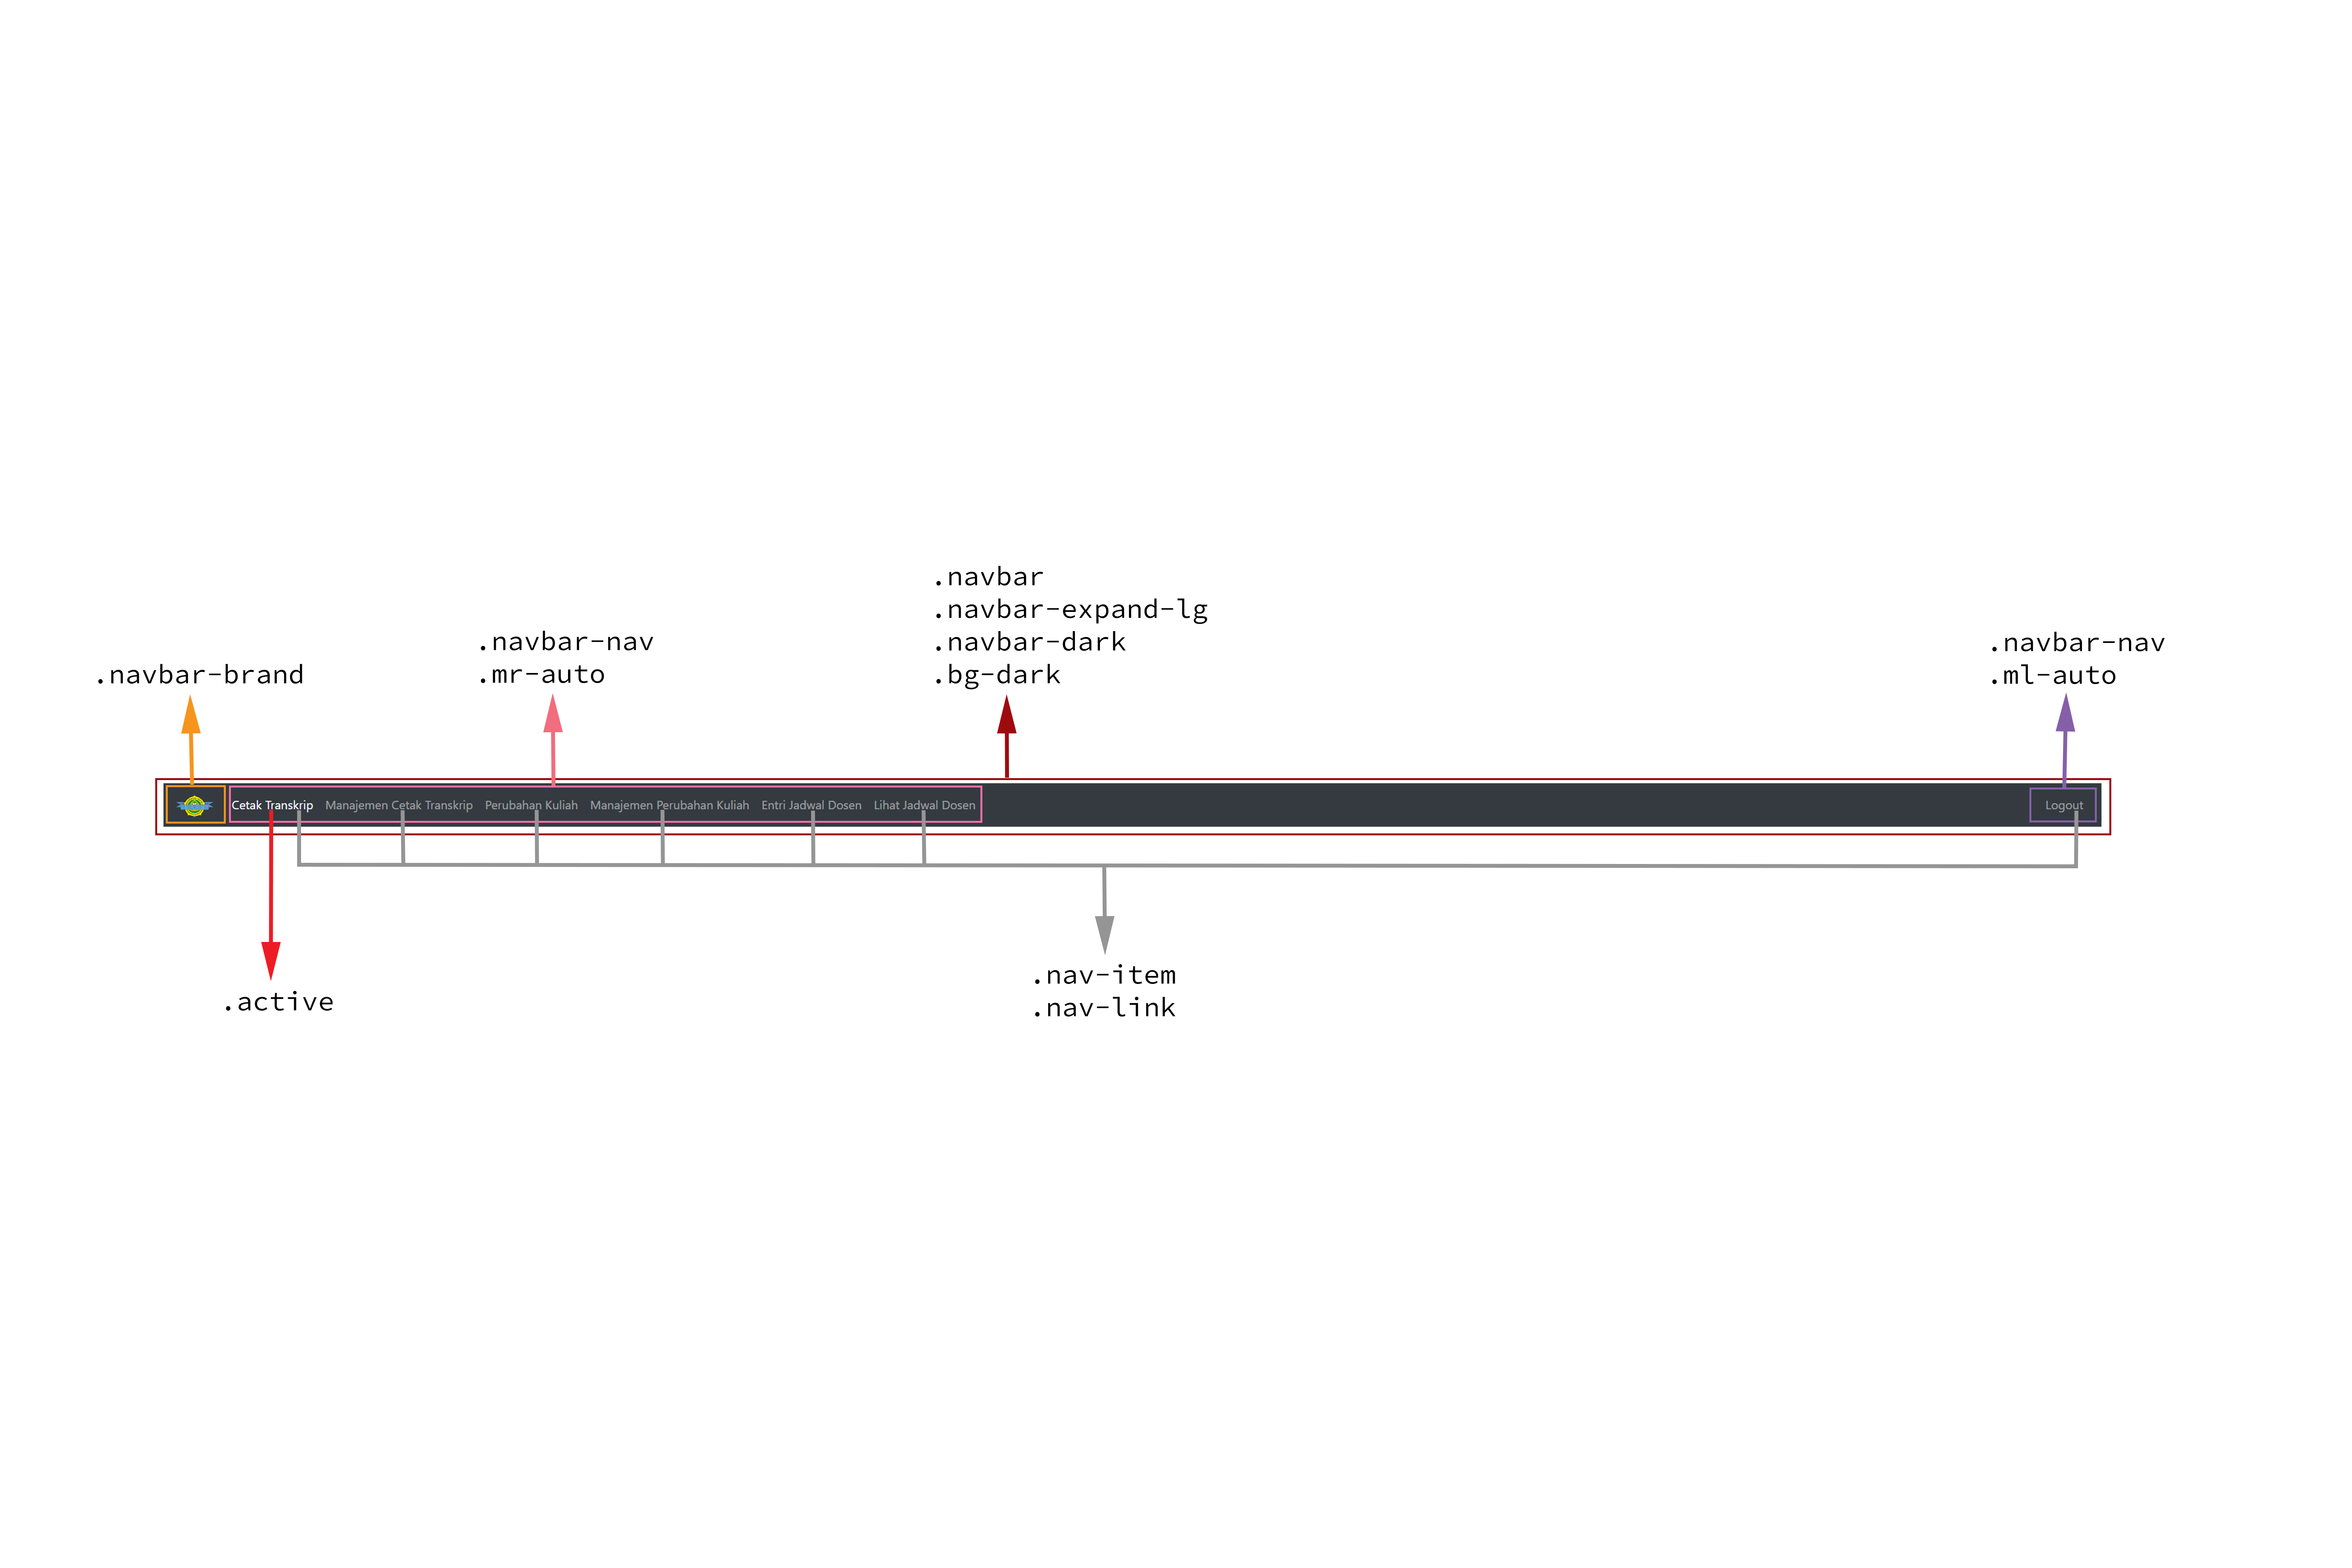
\includegraphics[width=\textwidth,height=\textheight,keepaspectratio]{bootstrap/konversi_navbar.png}  
	\caption{Konversi Tampilan Login} 
\end{figure}
Navigation bar diaplikasin untuk keseluruhan tampilan website, pada layar medium dan small daftar menu akan berubah menjadi ikon menu.
Kelas yang digunakan adalah sebagai berikut.
\begin{itemize}
	\item \texttt{.top-bar}	: Menu akan terletak pada bagian atas dari halaman.	
	\item \texttt{.menu}	: Kelas merupakan fondasi untuk membangun komponen dalam sebuah navigasi seperti daftar menu, judul dan letak menu.
	\item \texttt{.menu-active}: Kelas untuk menandakan menu yang dipilih user.
	\item \texttt{.menu-text}: Kelas untuk menyelaraskan nama menu berbentuk teks agar sejajar dengan \textit{navigation bar}.	
	\item \texttt{.top-bar-left}: Kelas yang mengatur daftar menu disebelah kiri.
	\item \texttt{.top-bar-right}: Kelas yang mengatur daftar menu disebelah kanan.
\end{itemize} \noindent \\
\begin{figure} [H]
	\centering  
	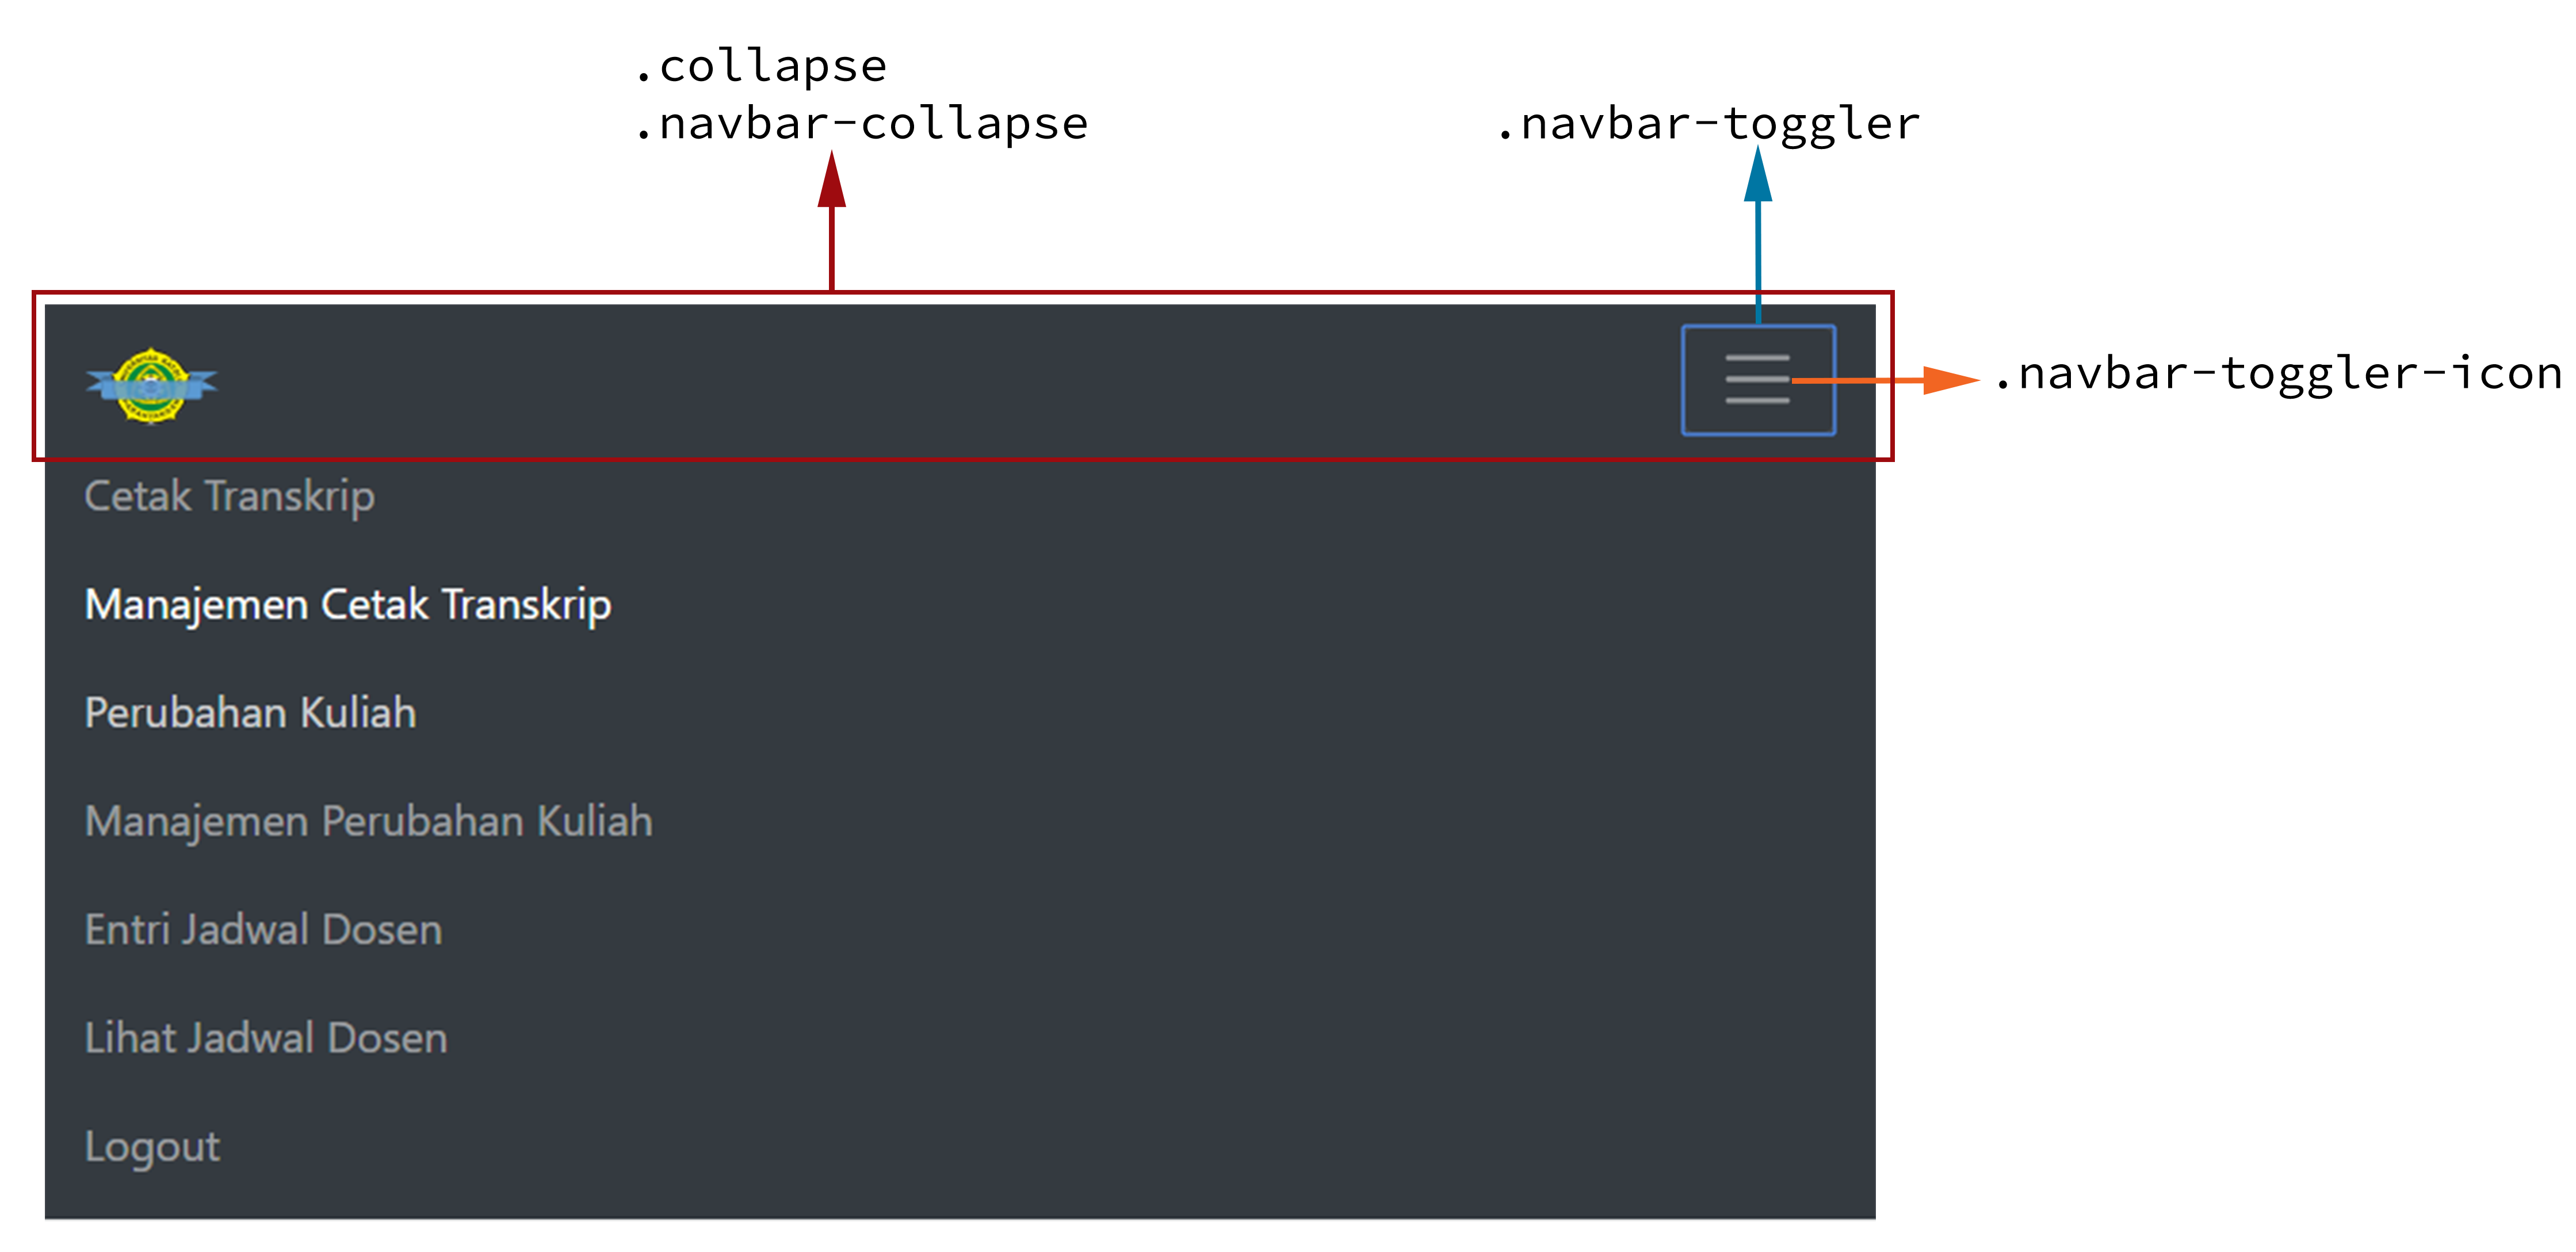
\includegraphics[width=\textwidth,height=\textheight,keepaspectratio]{bootstrap/konversi_small_navbar.png}  
	\caption{Analisis Tampilan Login pada layar Medium dan Small} 
\end{figure}
Kemudian pada layar \textit{mobile} digunakan komponen \textit{Advanced Layout} dimana daftar menu akan dalam mode \textit{hide}.
\begin{itemize}	
	\item \texttt{.title-bar} \texttt{data-responsive-toggle}: Inisiasi untuk membuat navigasi menu yang responsif. 
	\item \texttt{.menu-icon}: Kelas untuk membuat icon menu.
	\item \texttt{.title-bar-title}	: Logo digunakan untuk judul website BlueTape, sehingga akan terletak pada bagian kanan dari \textit{navigation bar}.
	%belum ada di analisis
	\item \texttt{data-toggle}: Atribut ini akan memanggil data yang disimpan dalam \texttt{data-toggle}.	
	\item \texttt{data-hide-for}: Atribut yang mengatur kapan menu navigasi akan responsif.
\end{itemize}

\subsection{Halaman Login}
\begin{figure} [H]
	\centering  
	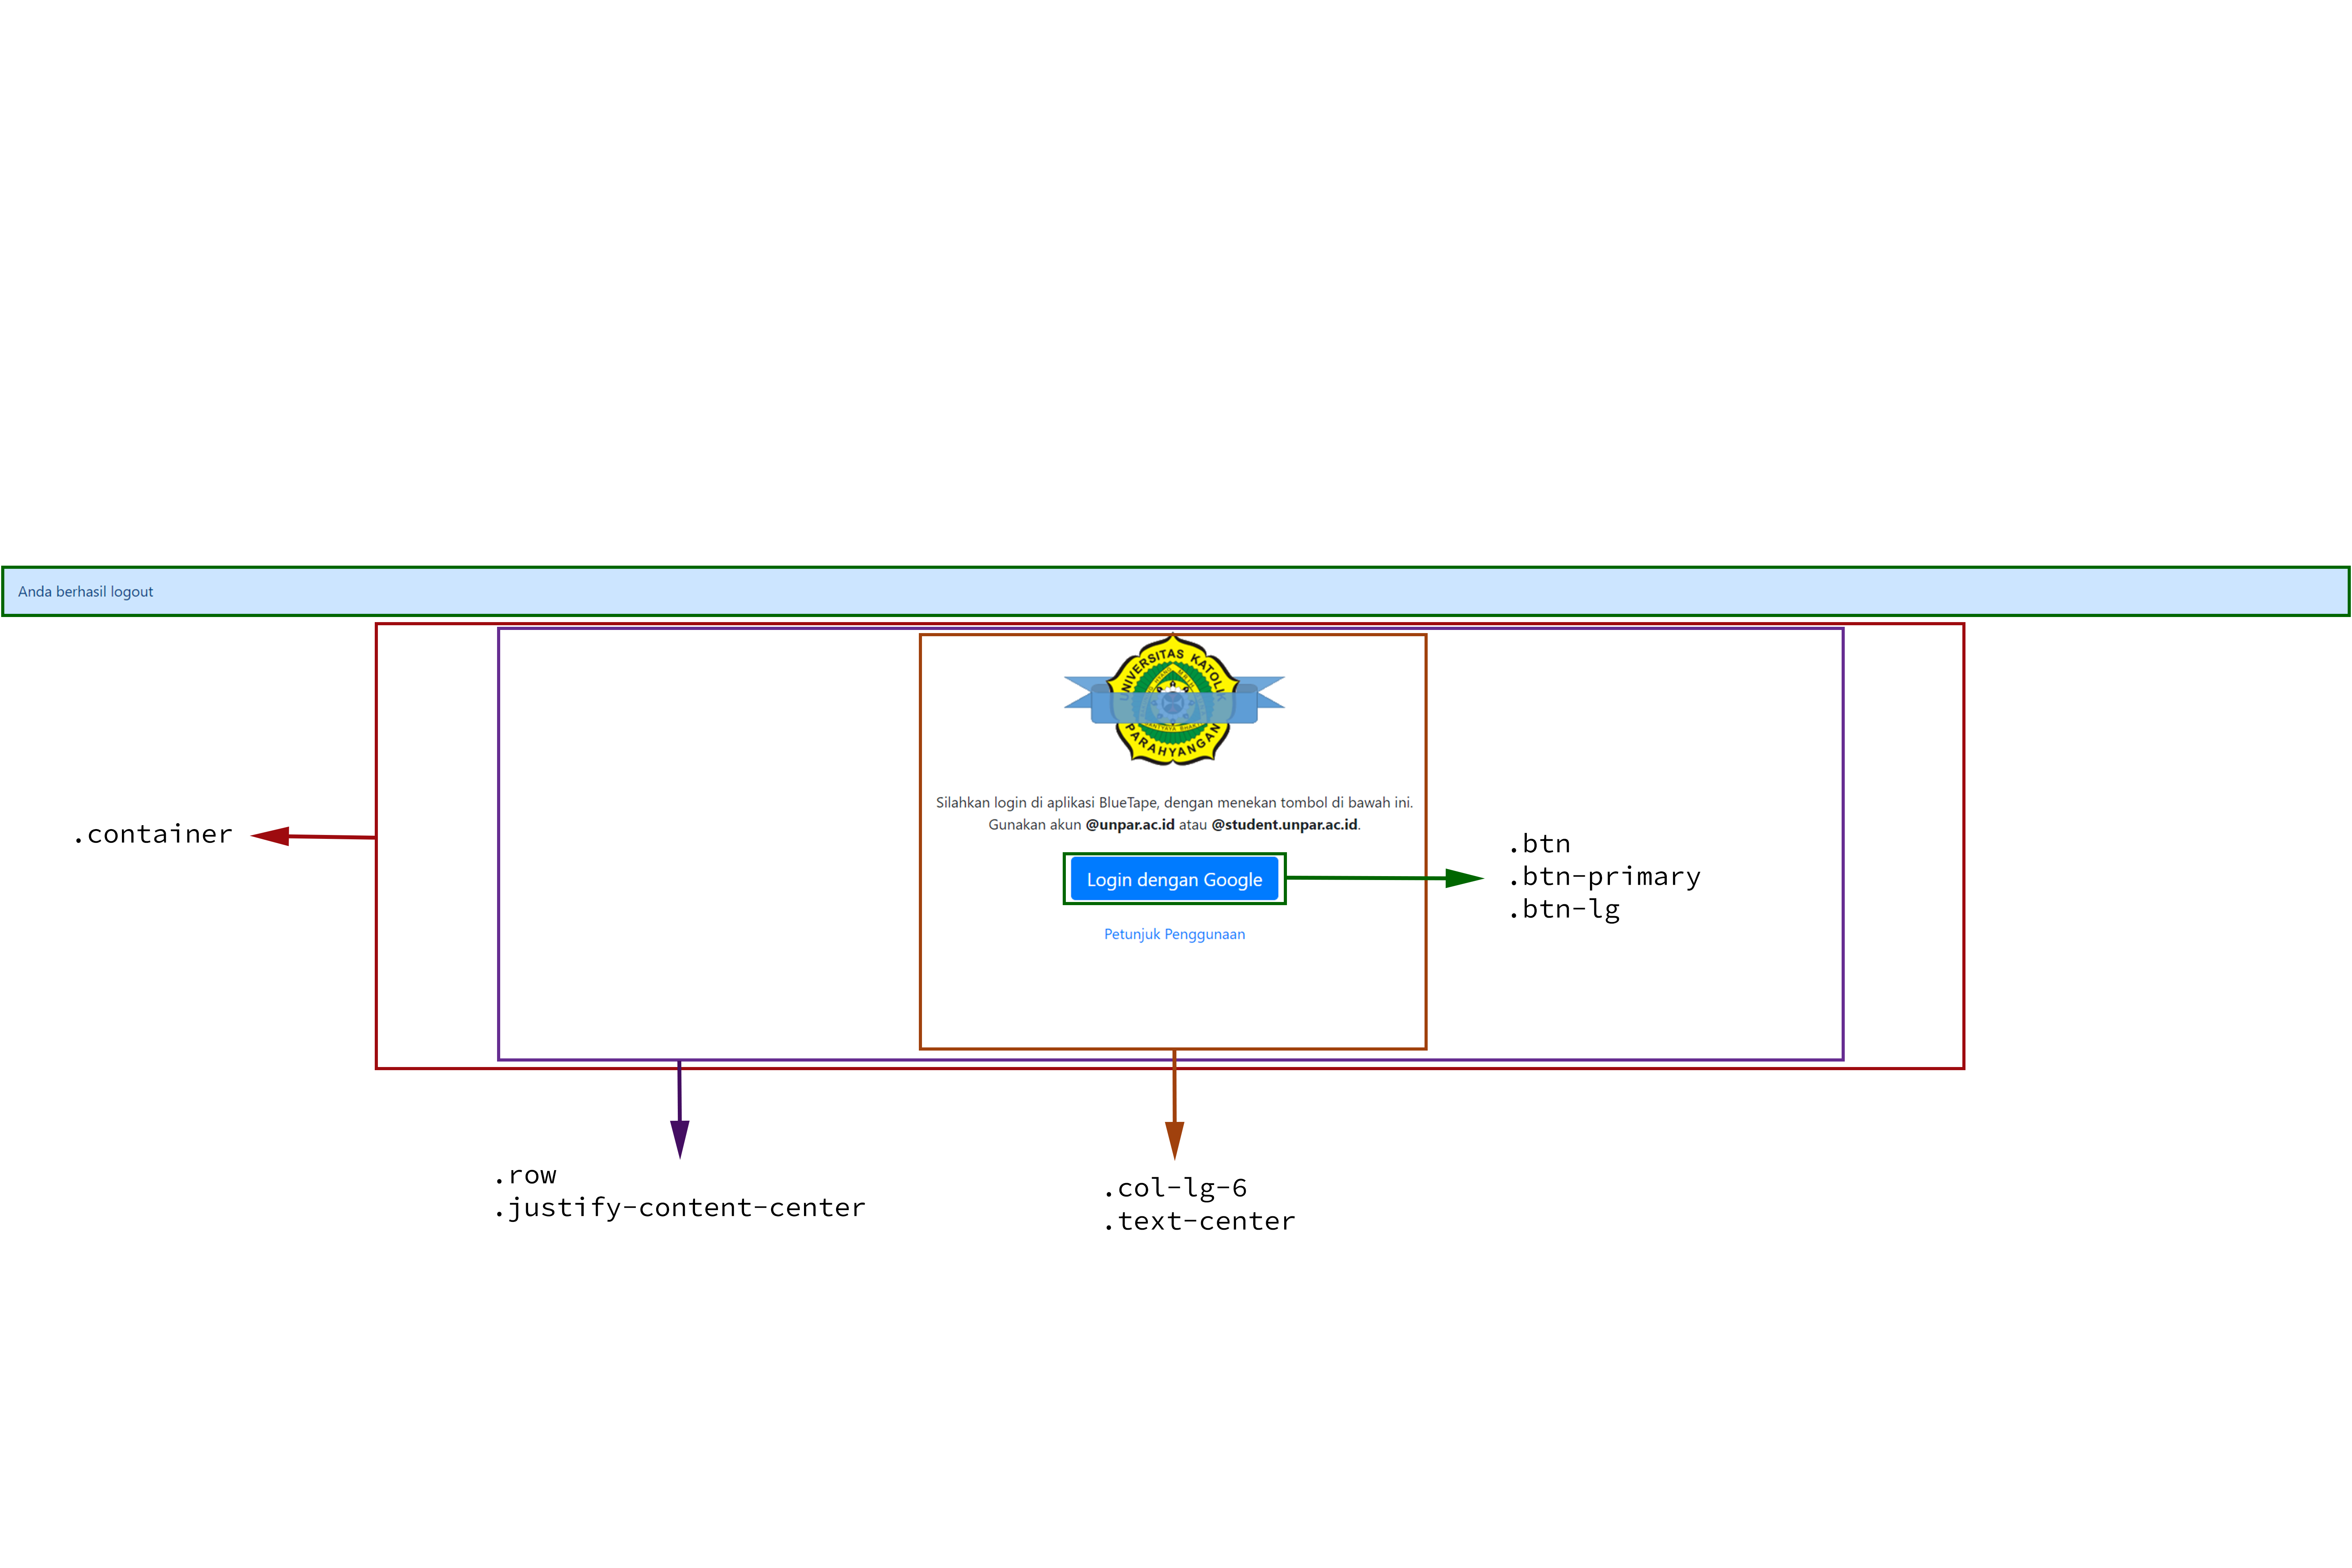
\includegraphics[width=\textwidth,height=\textheight,keepaspectratio]{bootstrap/konversi_tampilan_login.png}  
	\caption{Konversi Tampilan Login} 
\end{figure} \noindent \\
Kelas yang digunakan dalam halaman ini sebagai berikut:
\begin{itemize}
	%posisi large-centered, .large-6 salah
	\item \texttt{.row, .large-6, .column}: Konten akan terletak sejajar secara horizontal.
	\item \texttt{.text-center}: Kalimat login terletak ditengah container.
	\item \texttt{.button expnad}: Tombol akan memiliki panjang yang menyesuaikan lebar konten.
	\item Callout]: Terdapat dua jenis kelas yang dipakai
	\begin{itemize}
		\item.callout alert	: Notifikasi bahwa user harus login untuk mengakses website.
		\item.callout primary	: Notifikasi bahwa user berhasil logout.
	\end{itemize}
	
\end{itemize}

\subsection{Halaman Cetak Transkrip}
\subsubsection{Halaman Utama}

\begin{figure} [H]
	\centering  
	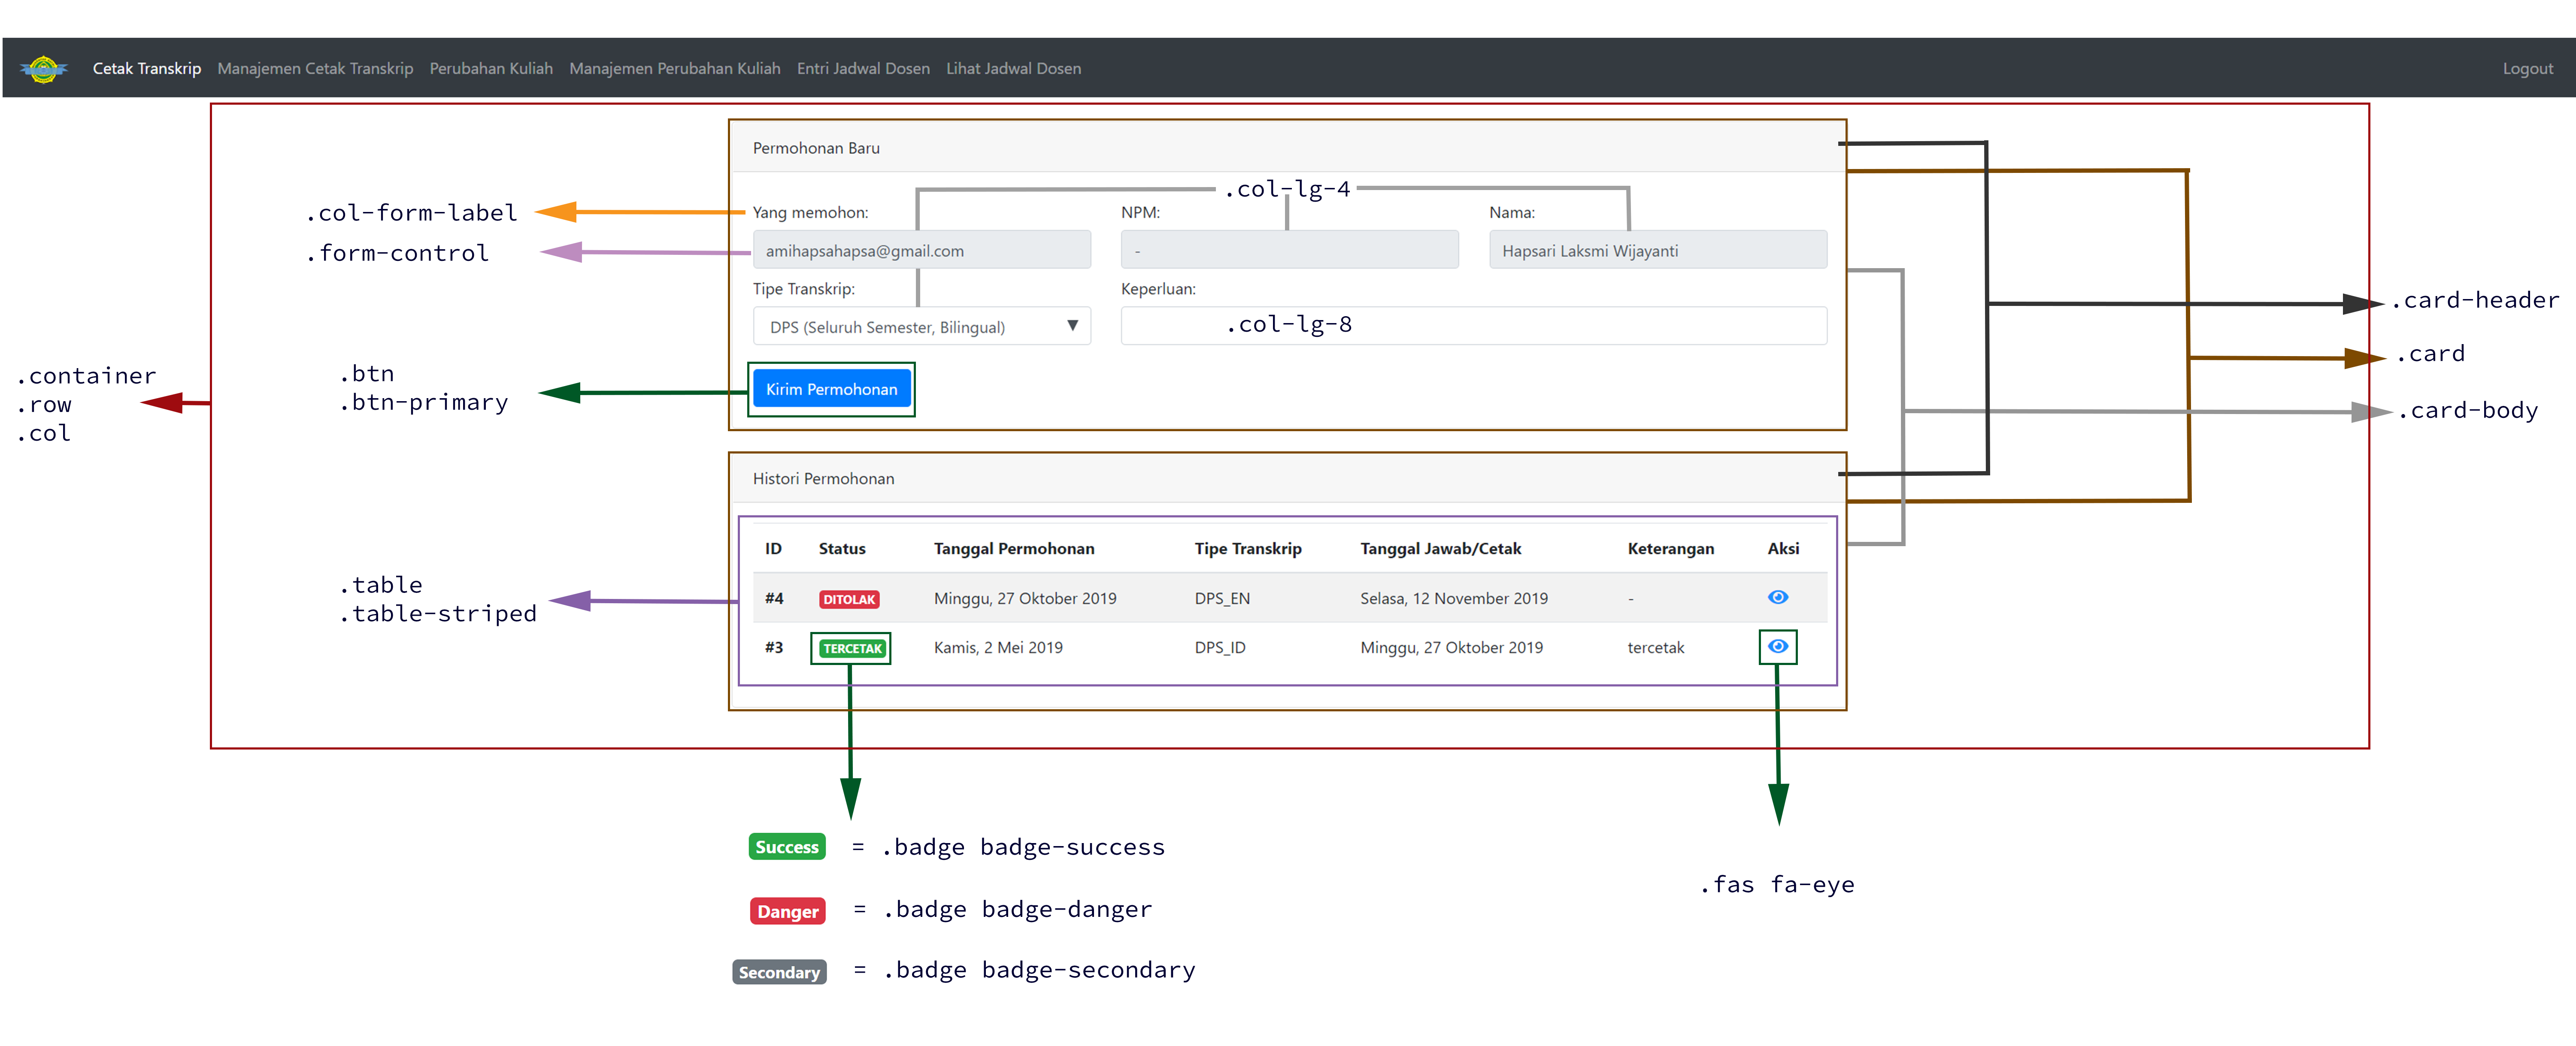
\includegraphics[width=\textwidth,height=\textheight,keepaspectratio]{bootstrap/konversi_tampilan_cetak_transkrip.png}
	\caption{Konversi Halaman Cetak Transkrip} 
\end{figure}
\begin{itemize}
	\item \texttt{.row}: Kelas ini memiliki dua fungsi sebagai container konten dan mengatur beberapa \textit{field-form} menjadi satu baris. 
	\item \texttt{.medium-12 column}: Mengatur agar pada layar medium, semua konten akan selebar 12 grid.
	\item \texttt{.callout}: Untuk membuat border yang memisahkan konten permohonan baru dan histori permohonan.
	\item \texttt{.stack}: Jenis tabel yang digunakan tabel histori permohonan, sehingga pada layar medium tabel akan tersusun secara bertumpuk.
	\item \texttt{.fas fa-eye}: Ikon Font Awesome yang digunakan untuk link ke modal lihat.
	\item \texttt{.button}: Jenis kelas yang digunakan pada tombol `Kirim Permohonan'
	\item \texttt{.stack}
	\item Label: Terdiri dari tiga jenis kelas:
	\begin{itemize}
		\item \texttt{.label success}: Label untuk transkrip yang telah tercetak
		\item \texttt{.label alert}: Label untuk transkrip yang gagal tercetak
		\item \texttt{.label secondary}: Label untuk transkrip yang belum tercetak
	\end{itemize}
	
\end{itemize}
%Modal: eye
\subsubsection{Modal}
Ikon eye akan menampilkan sebuah modal yang menampilkan Detail Permohonan berdasarkan ID yang tercatat.
\begin{figure} [H]
	\centering  
	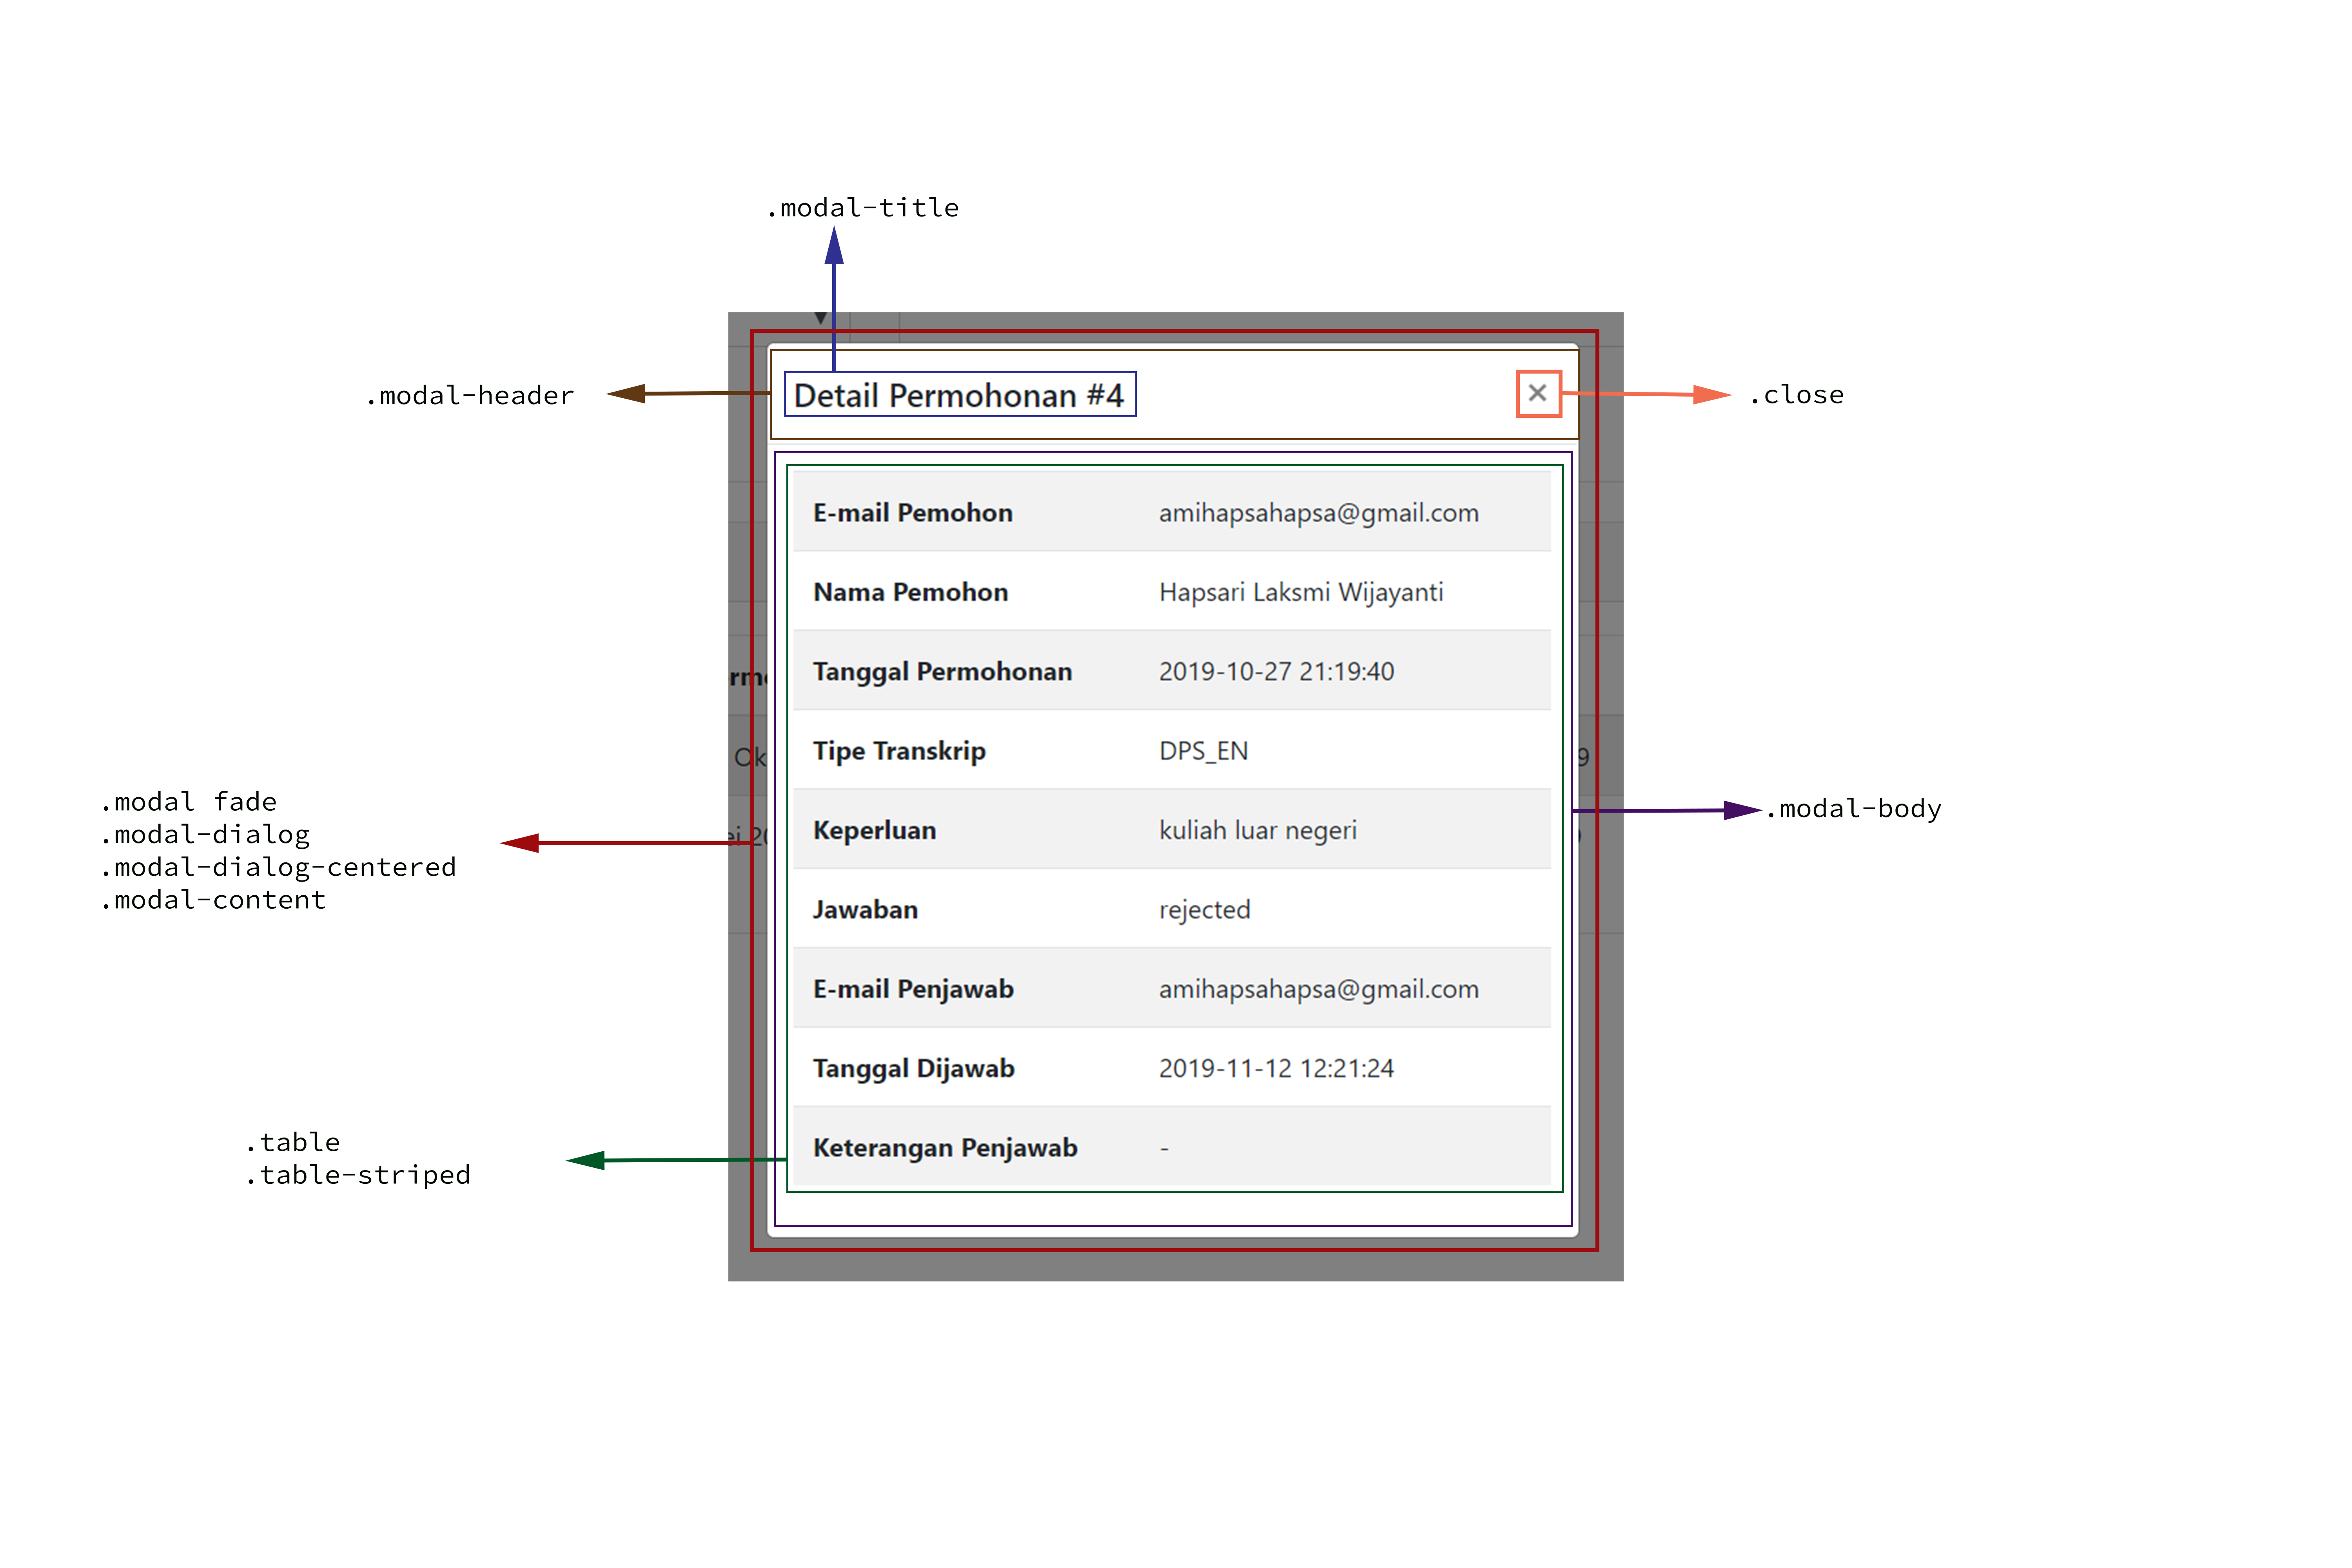
\includegraphics[width=\textwidth,height=\textheight,keepaspectratio]{bootstrap/konversi_modal_lihat_cetak_transkrip.png}  
	\caption{Konversi Modal Lihat} 
\end{figure}

Komponen Modal terdiri dari:
\begin{itemize}
	\item \texttt{.reveal data-reveal}: Membuat modal yang menampung tabel detail permohonan.
	\item \texttt{.close-button data-close}: Menutup modal yang telah terbuka.
	\item \texttt{.stack}:	Membuat tabel detail permohonan.
\end{itemize}
\subsection{Halaman Manajemen Cetak Transkrip}
\subsubsection{Halaman Utama}
\begin{figure} [H]
	\centering  
	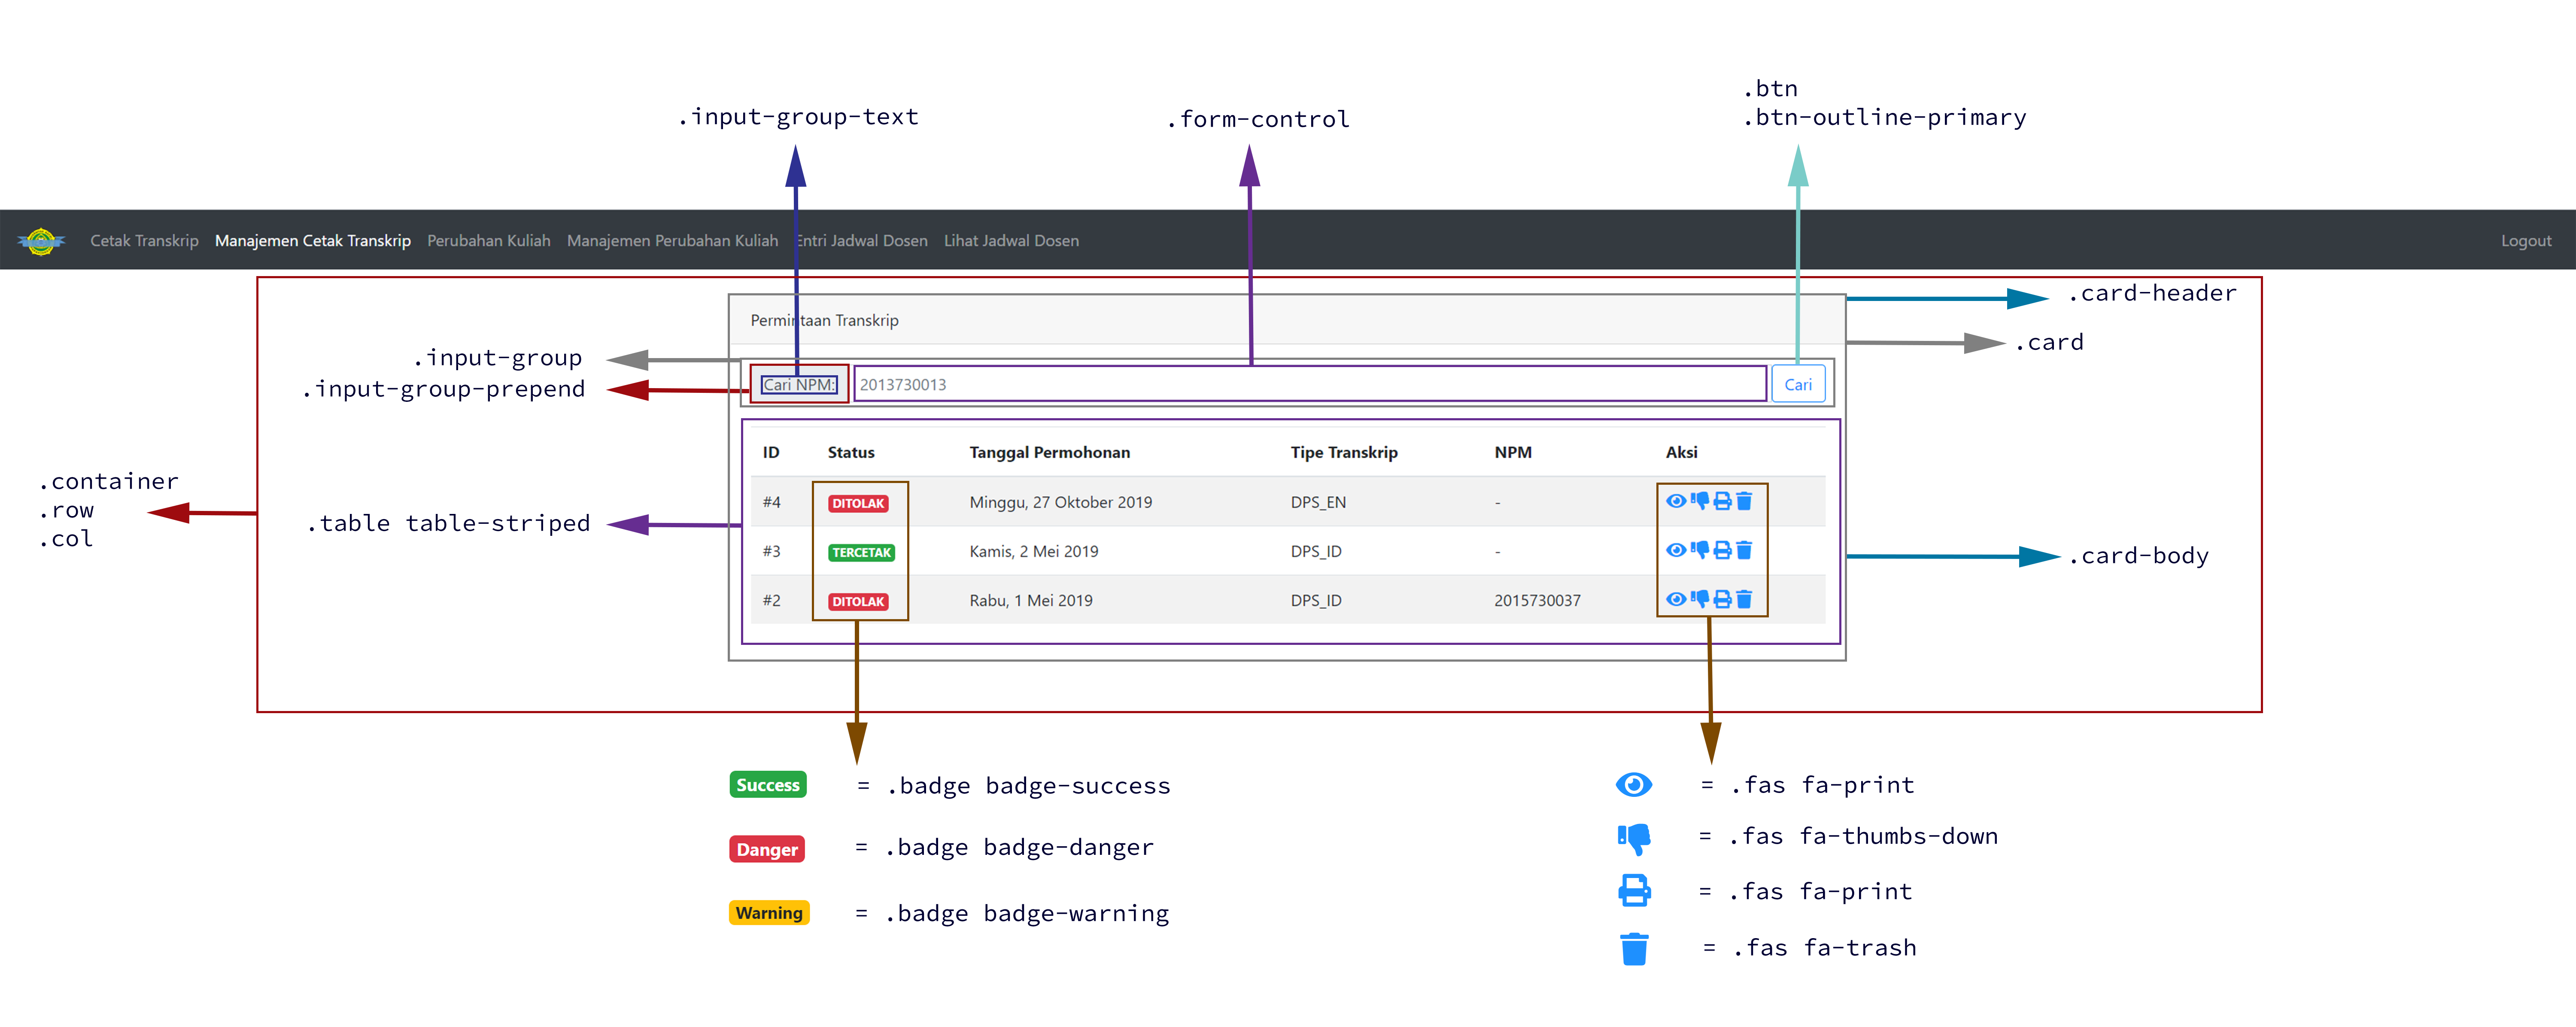
\includegraphics[width=\textwidth,height=\textheight,keepaspectratio]{bootstrap/konversi_tampilan_manajemen_cetak_transkrip.png}
	\caption{Konversi Manajemen Cetak Transkrip} 
\end{figure}
\begin{itemize}
	\item \texttt{.row}: Kelas ini memiliki dua fungsi sebagai container konten dan mengatur beberapa \textit{field-form} menjadi satu baris. 
	\item \texttt{.callout}: Untuk membuat border yang memisahkan konten permohonan baru dan histori permohonan.
	\item \texttt{.stack}: Jenis tabel yang digunakan tabel histori permohonan, sehingga pada layar medium tabel akan tersusun secara bertumpuk.
	\item Ikon Font Awesome yang terdiri dari 
	\begin{itemize}
		\item \texttt{.fas fa-eye}: Ikon untuk menuju modal lihat transkrip.
		\item \texttt{.fas fa-dislike}: Ikon untuk menuju modal tolak cetak transkrip.
		\item \texttt{.fas fa-print}: Ikon untuk menuju modal cetak transkrip.
		\item \texttt{.fas fa-trash}: Ikon untuk menuju hapus permitaan transkrip.
	\end{itemize}
	\item Label: Terdiri dari tiga jenis kelas:
	\begin{itemize}
		\item \texttt{.label success}: Label untuk transkrip yang telah tercetak
		\item \texttt{.label alert}: Label untuk transkrip yang gagal tercetak
		\item \texttt{.label warning}: Label untuk transkrip yang menunggu untuk tercetak
	\end{itemize}
	
\end{itemize}
%Modal: kecuali like
\begin{figure} [H]
	\centering  
	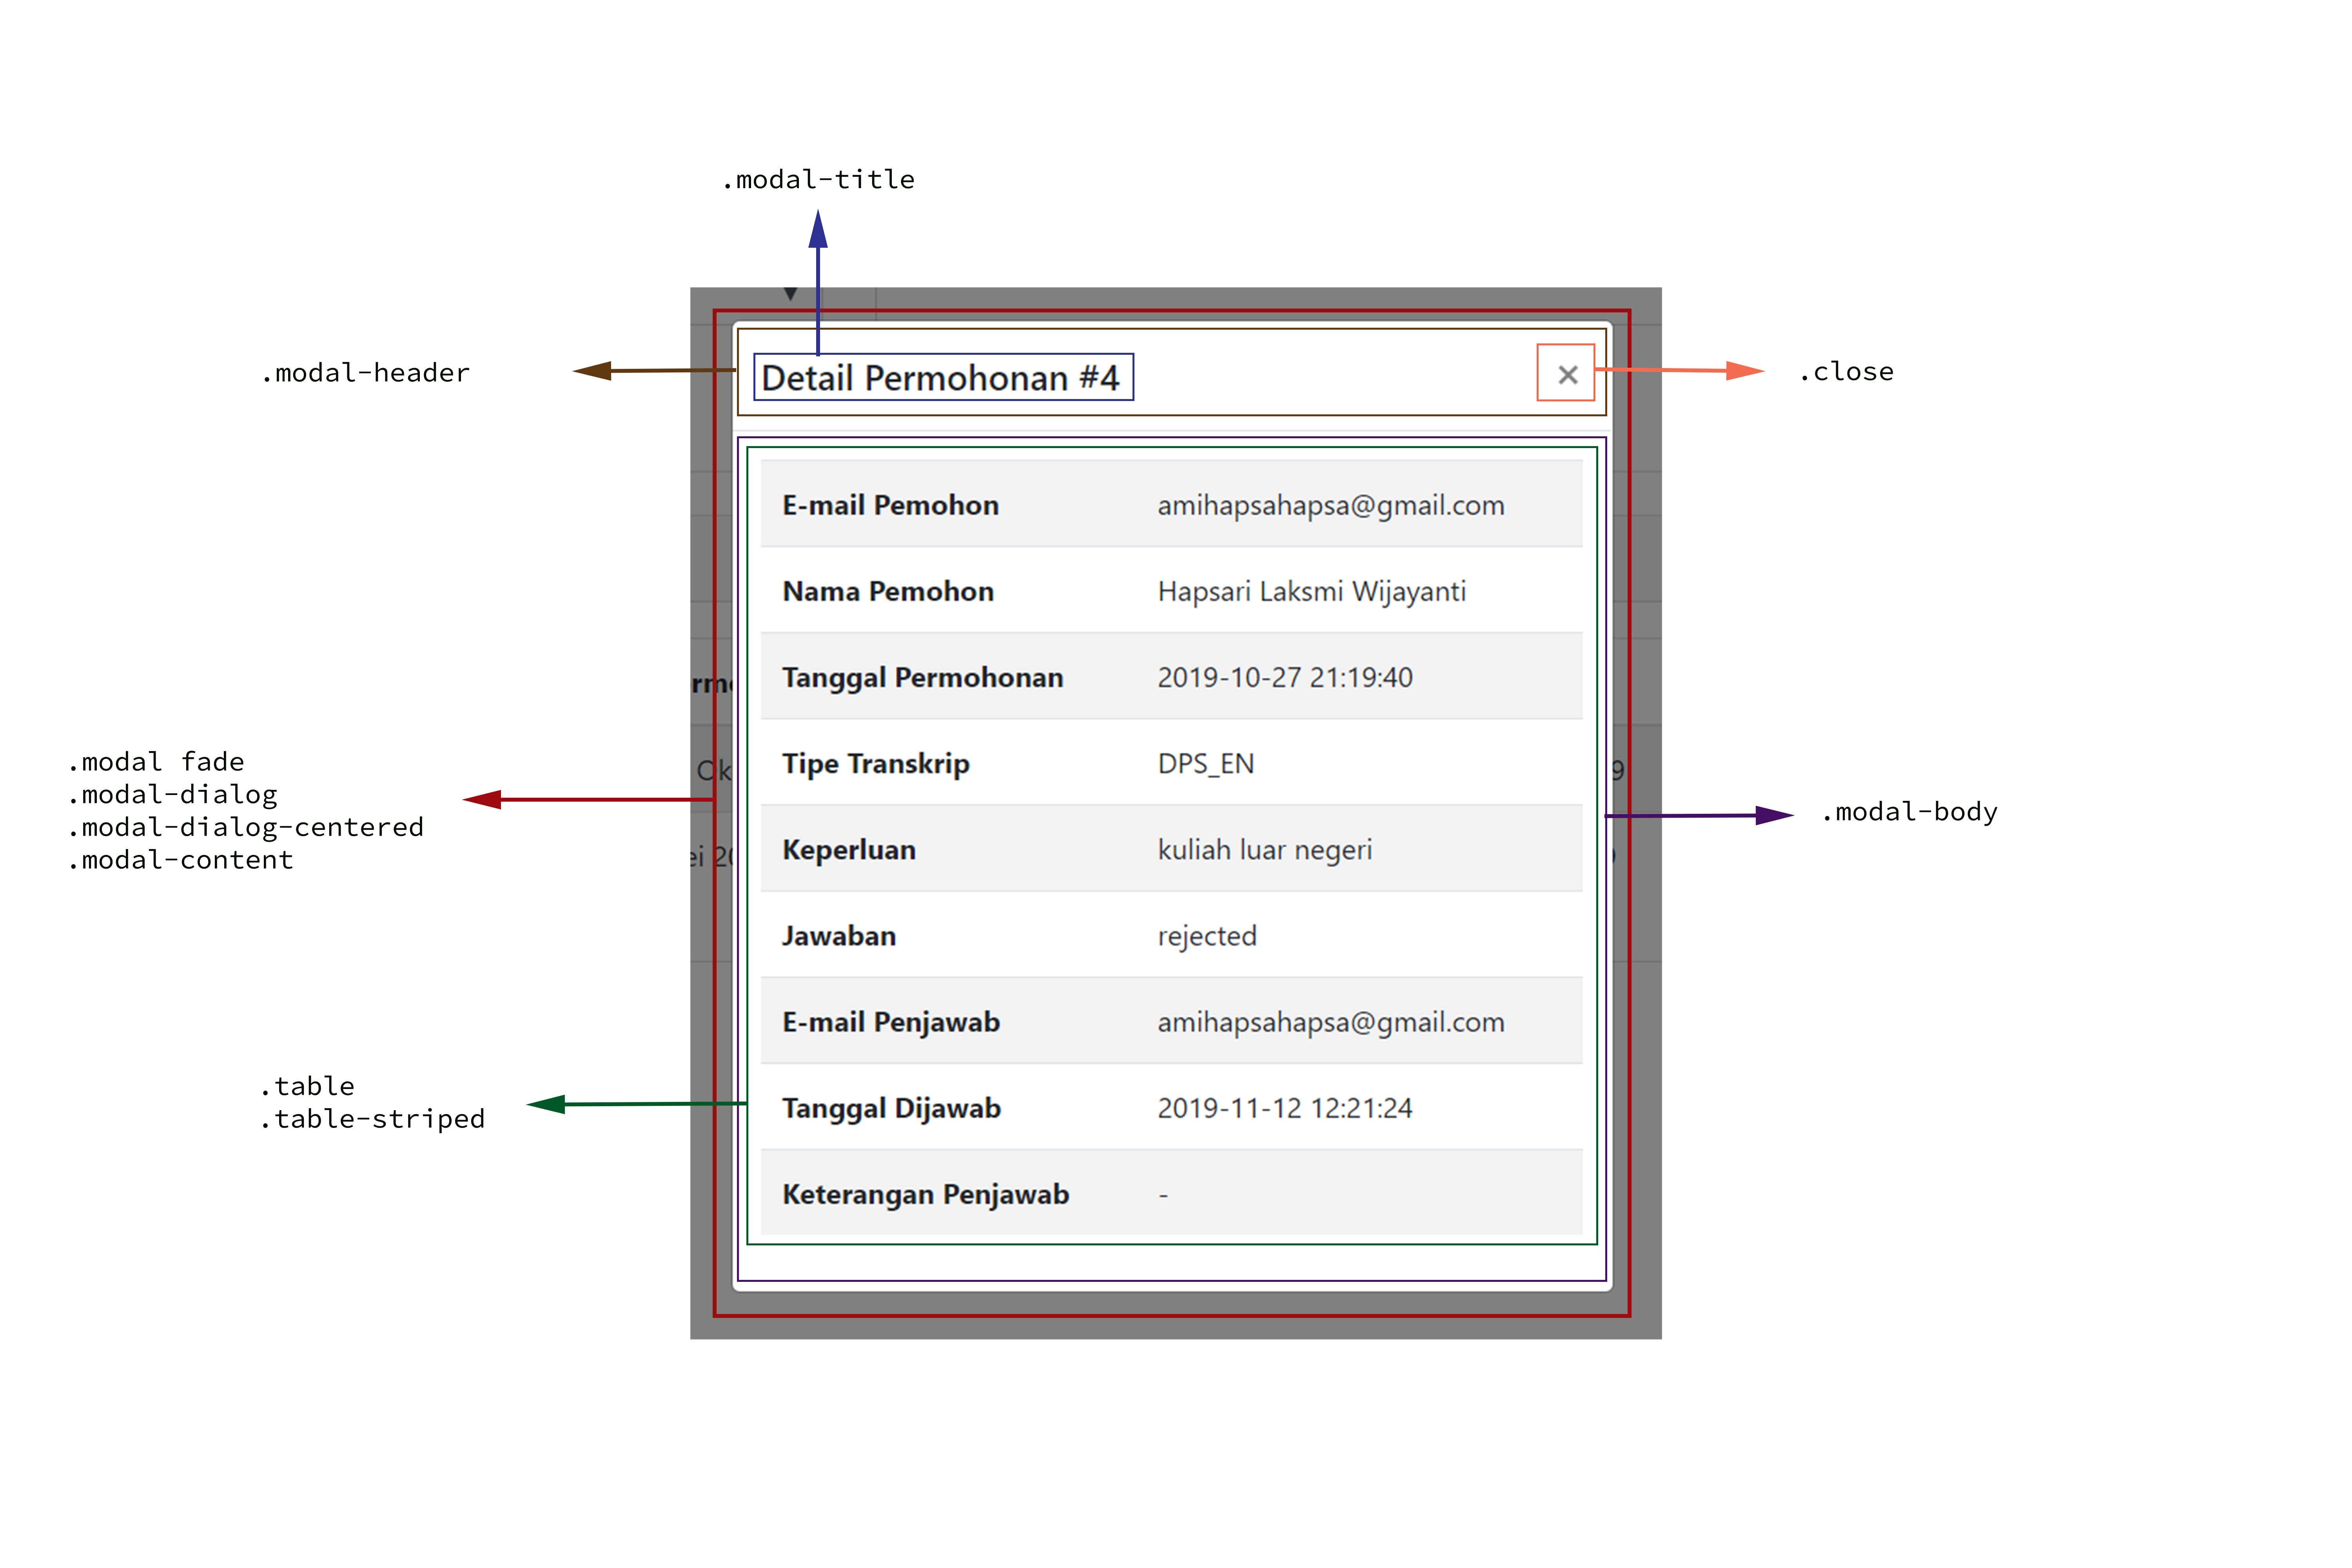
\includegraphics[width=\textwidth,height=\textheight,keepaspectratio]{bootstrap/konversi_modal_lihat_manajemen_cetak_transkrip.png}
	\caption{Konversi Modal Lihat} 
\end{figure}
\begin{figure} [H]
	\centering  
	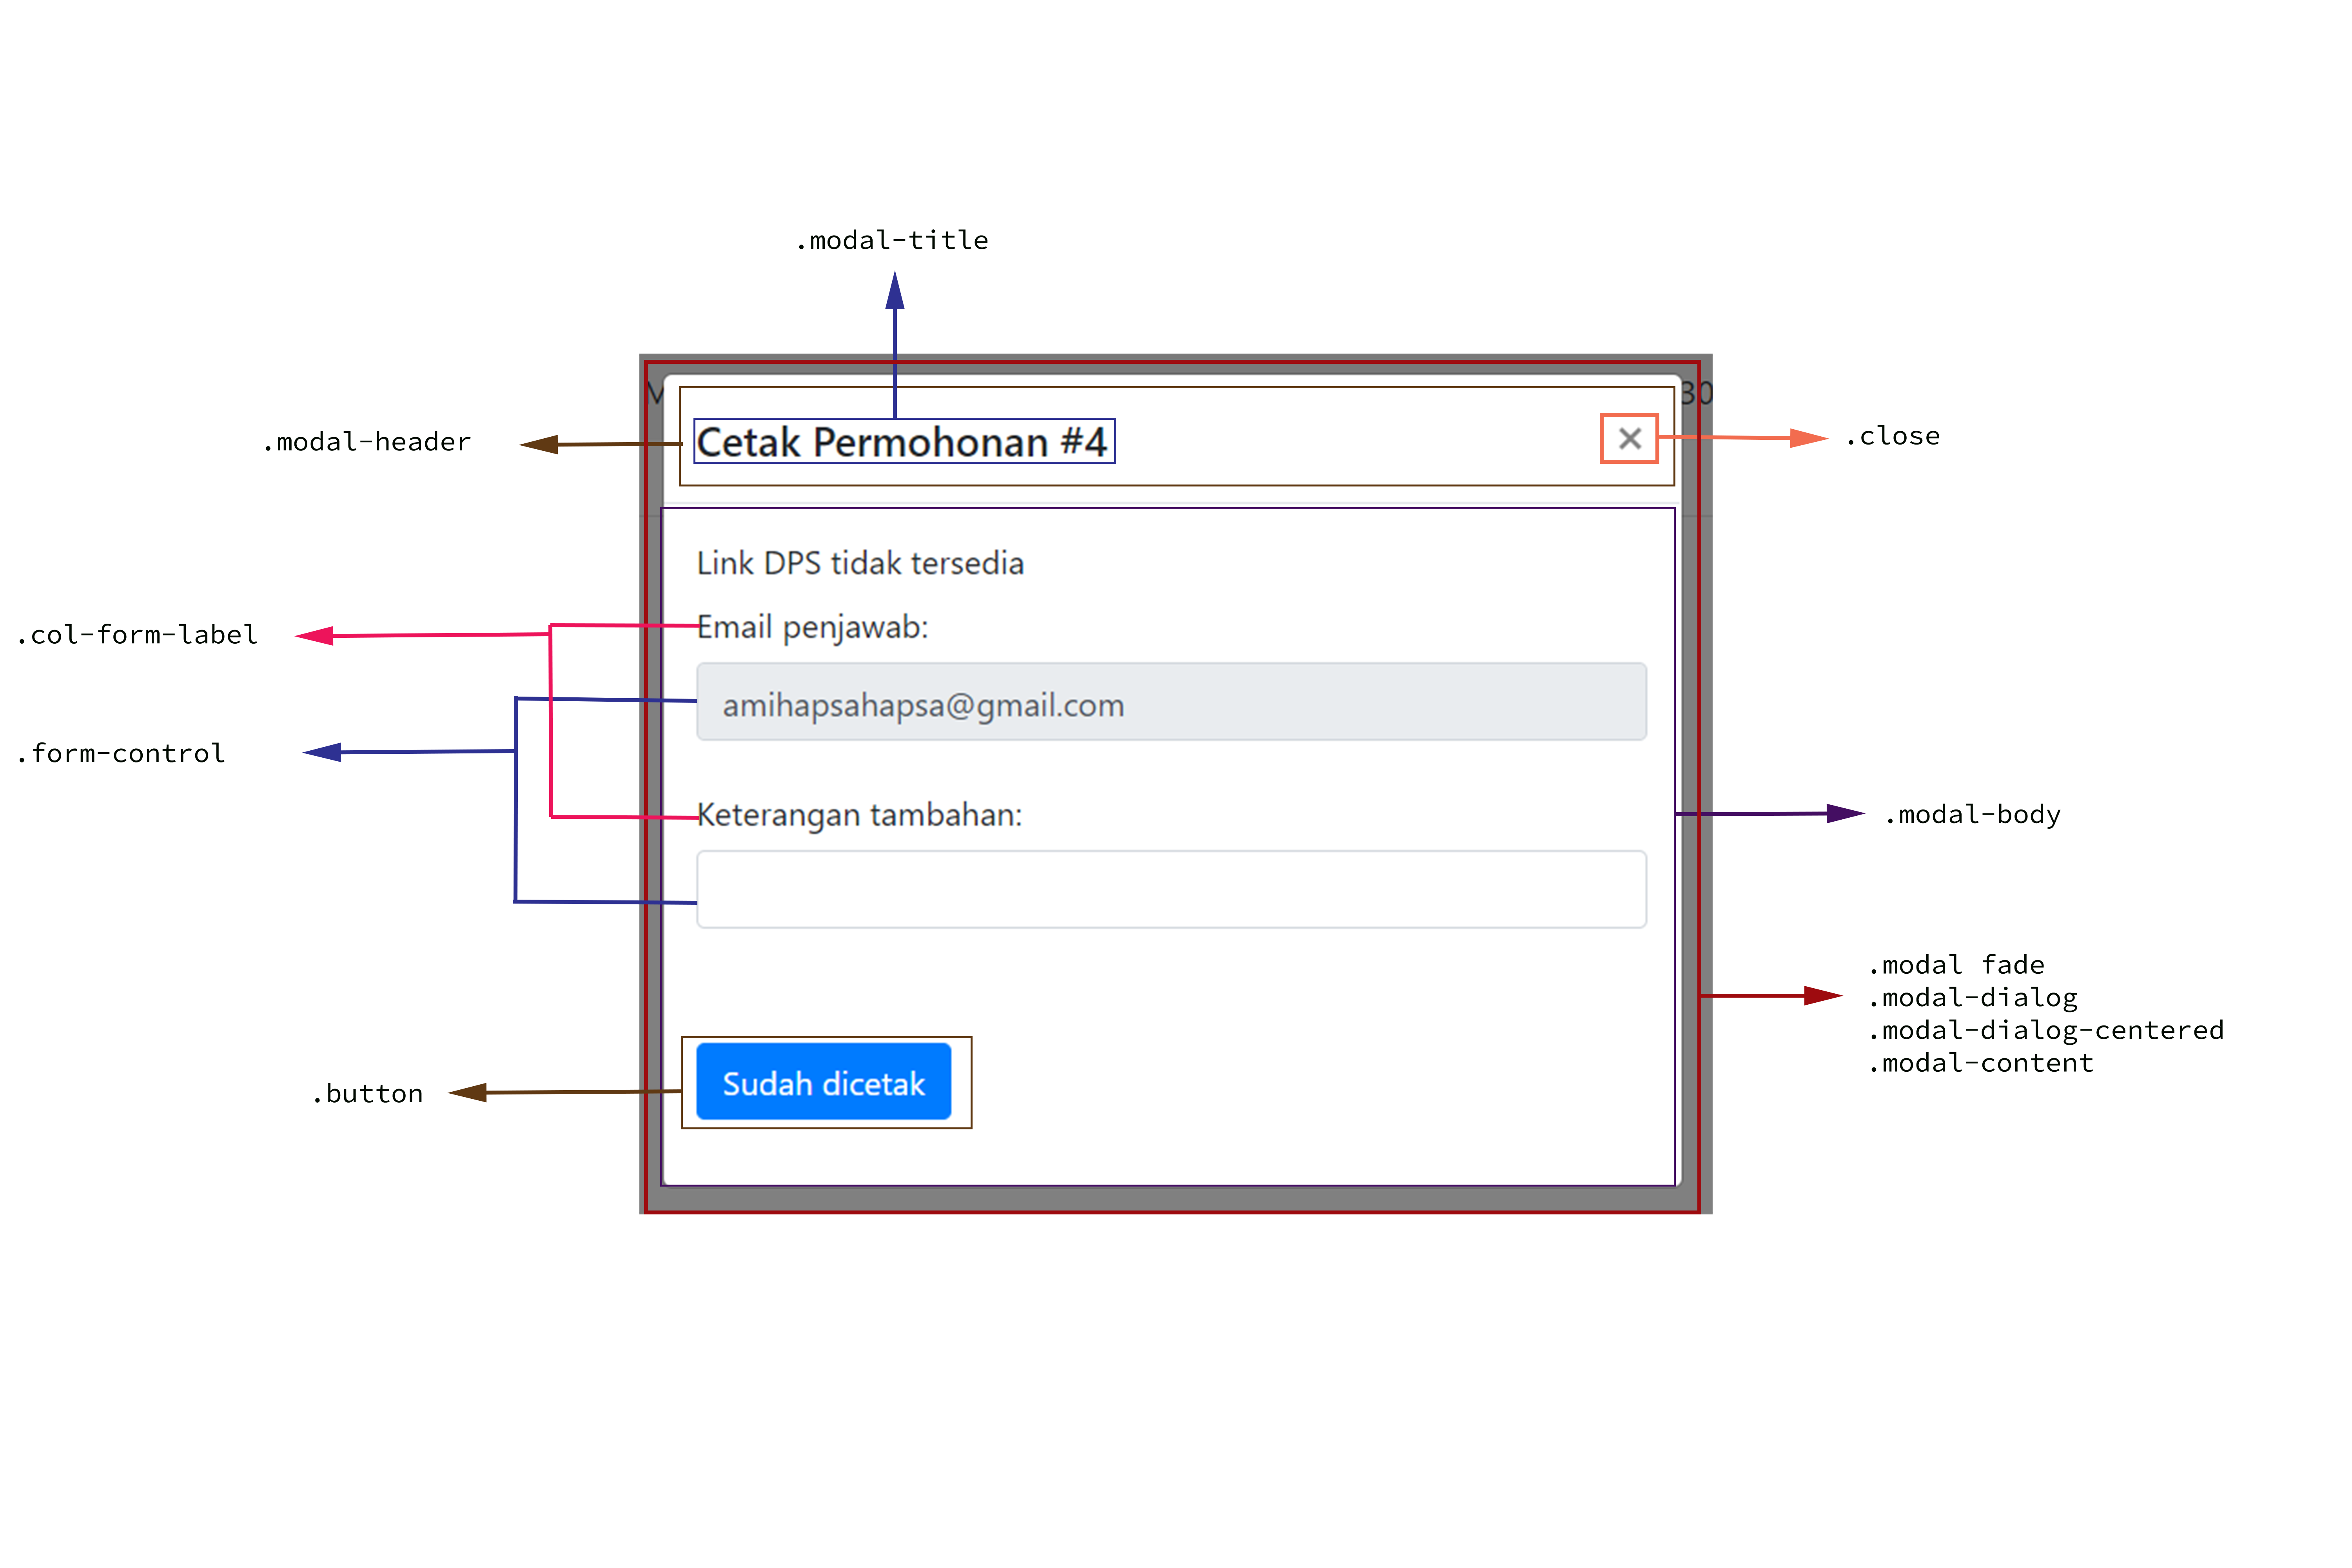
\includegraphics[width=\textwidth,height=\textheight,keepaspectratio]{bootstrap/konversi_modal_print_manajemen_cetak_transkrip.png}
	\caption{Konversi Modal Print} 
\end{figure}
\begin{figure} [H]
	\centering  
	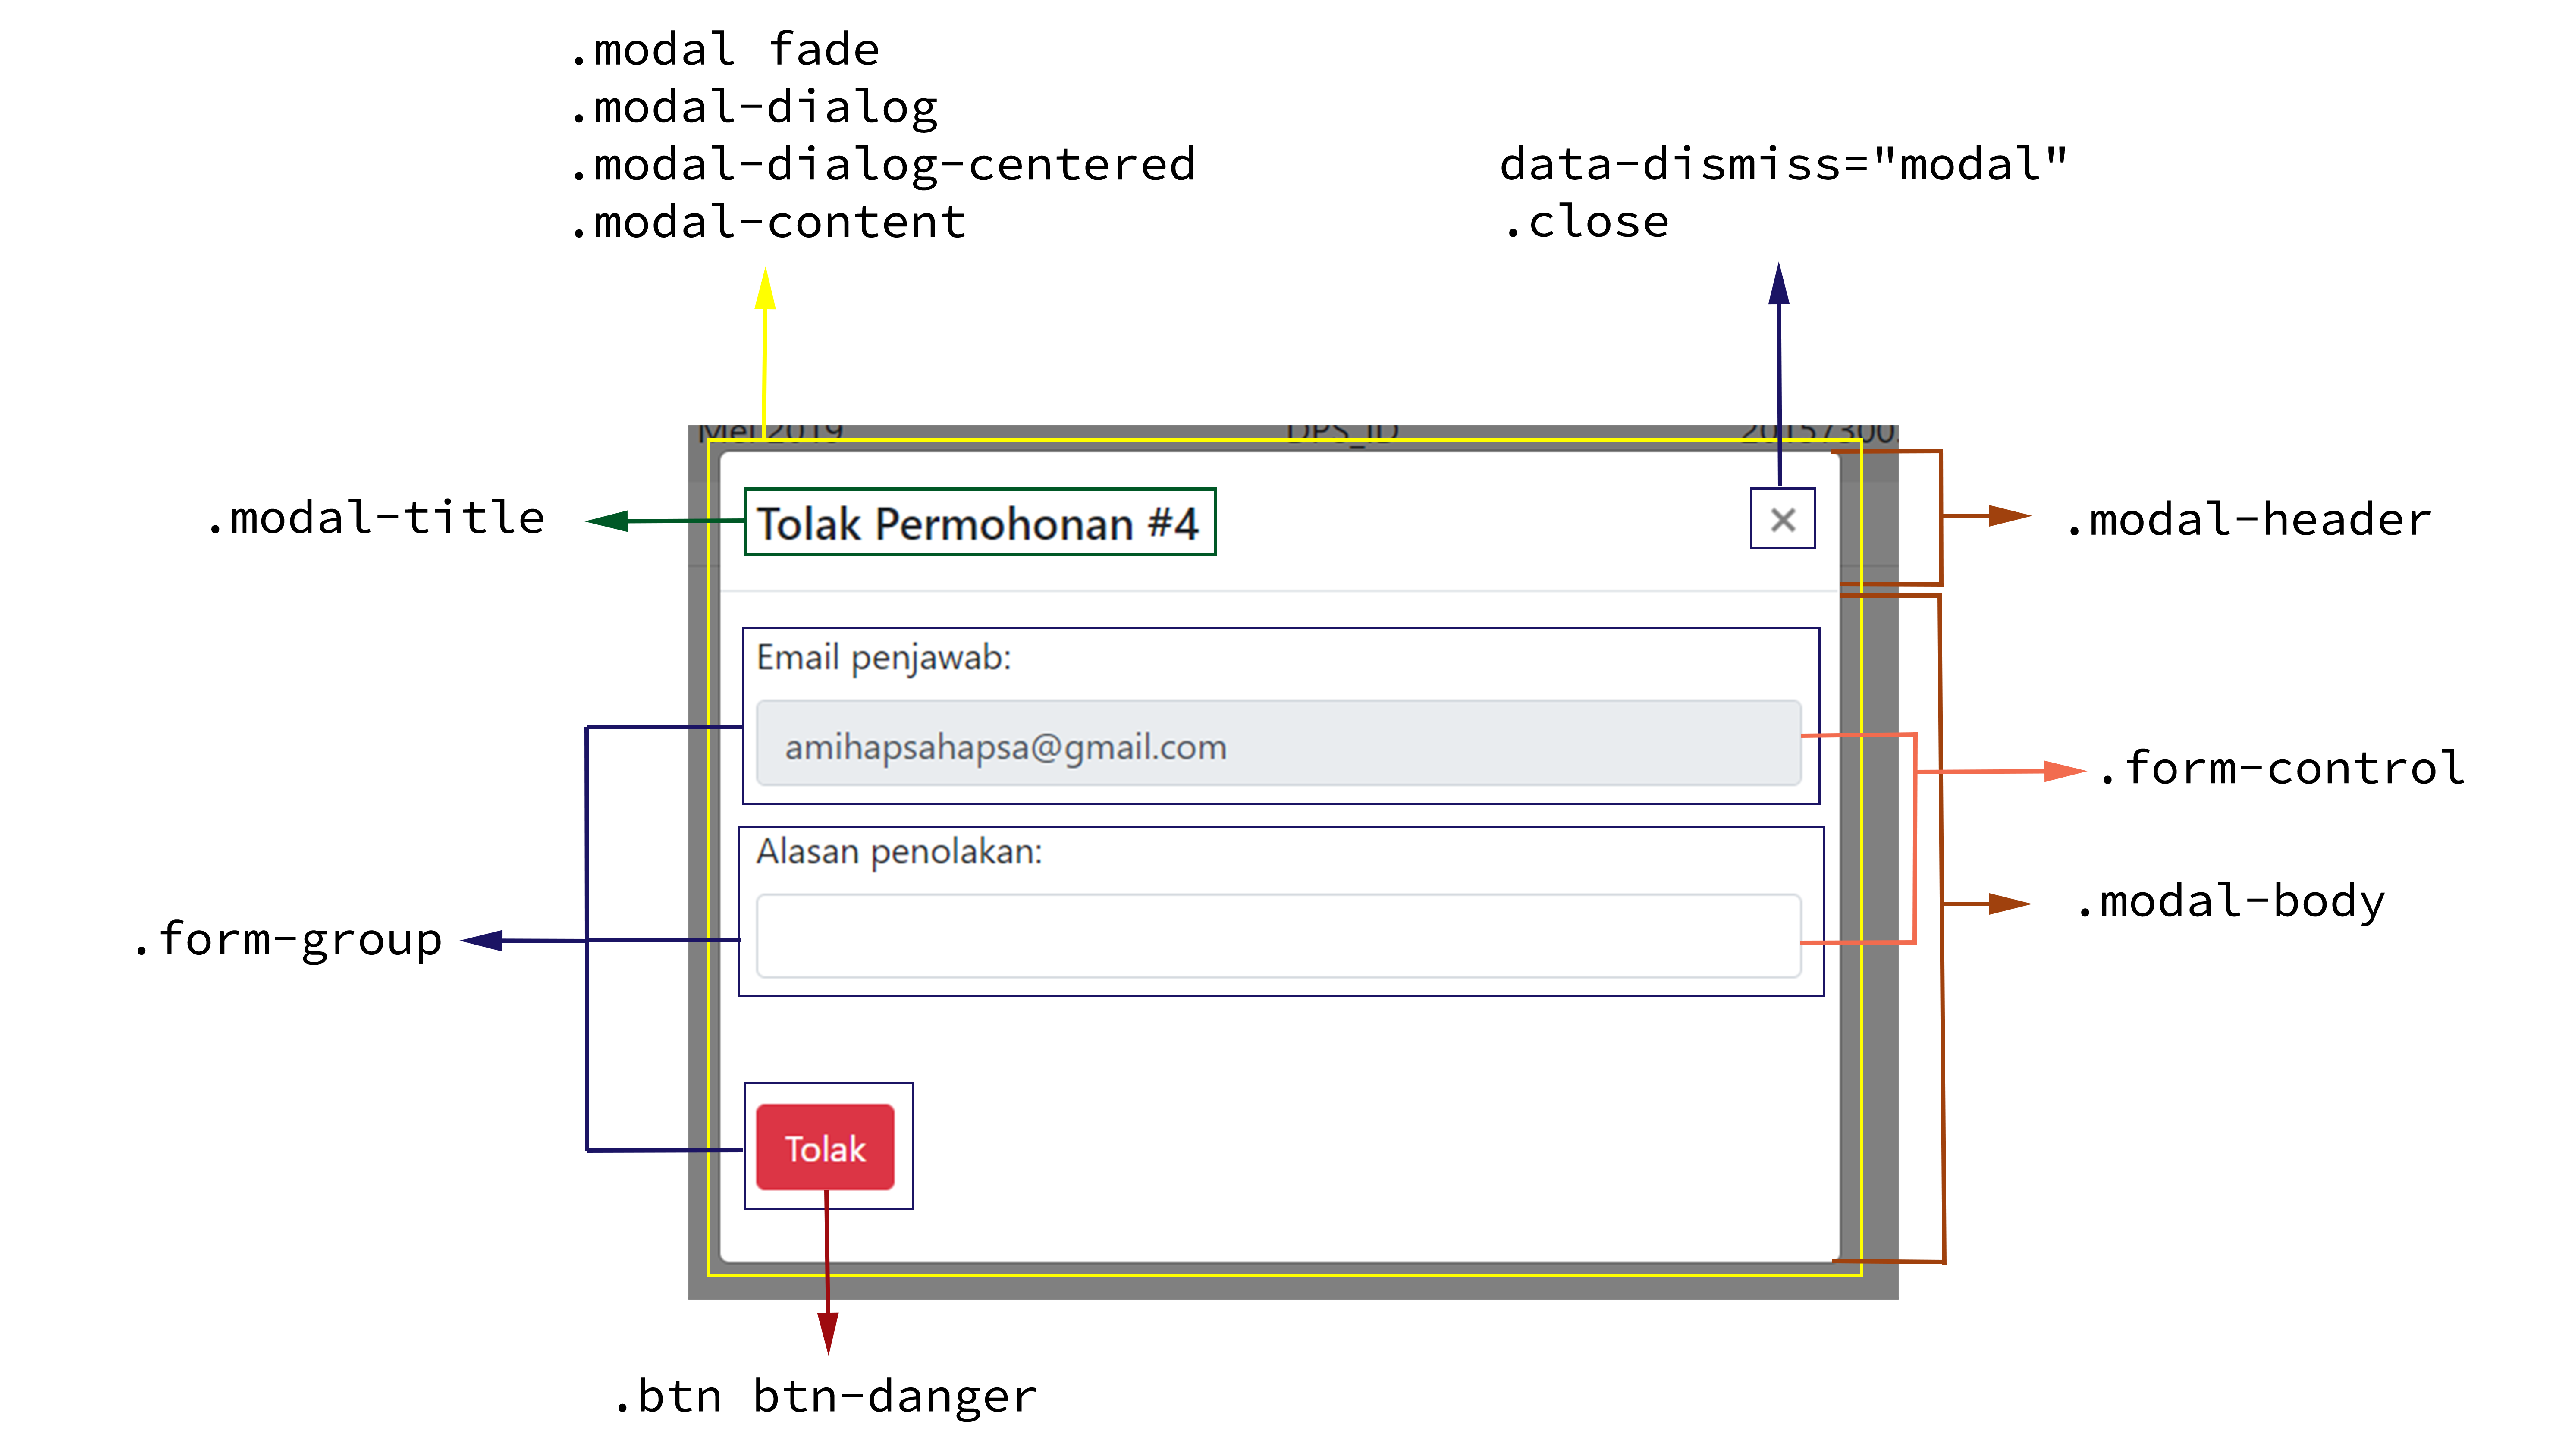
\includegraphics[width=\textwidth,height=\textheight,keepaspectratio]{bootstrap/konversi_modal_dislike_manajemen_cetak_transkrip.png}
	\caption{Konversi Modal Tolak} 
\end{figure}
\begin{figure} [H]
	\centering  
	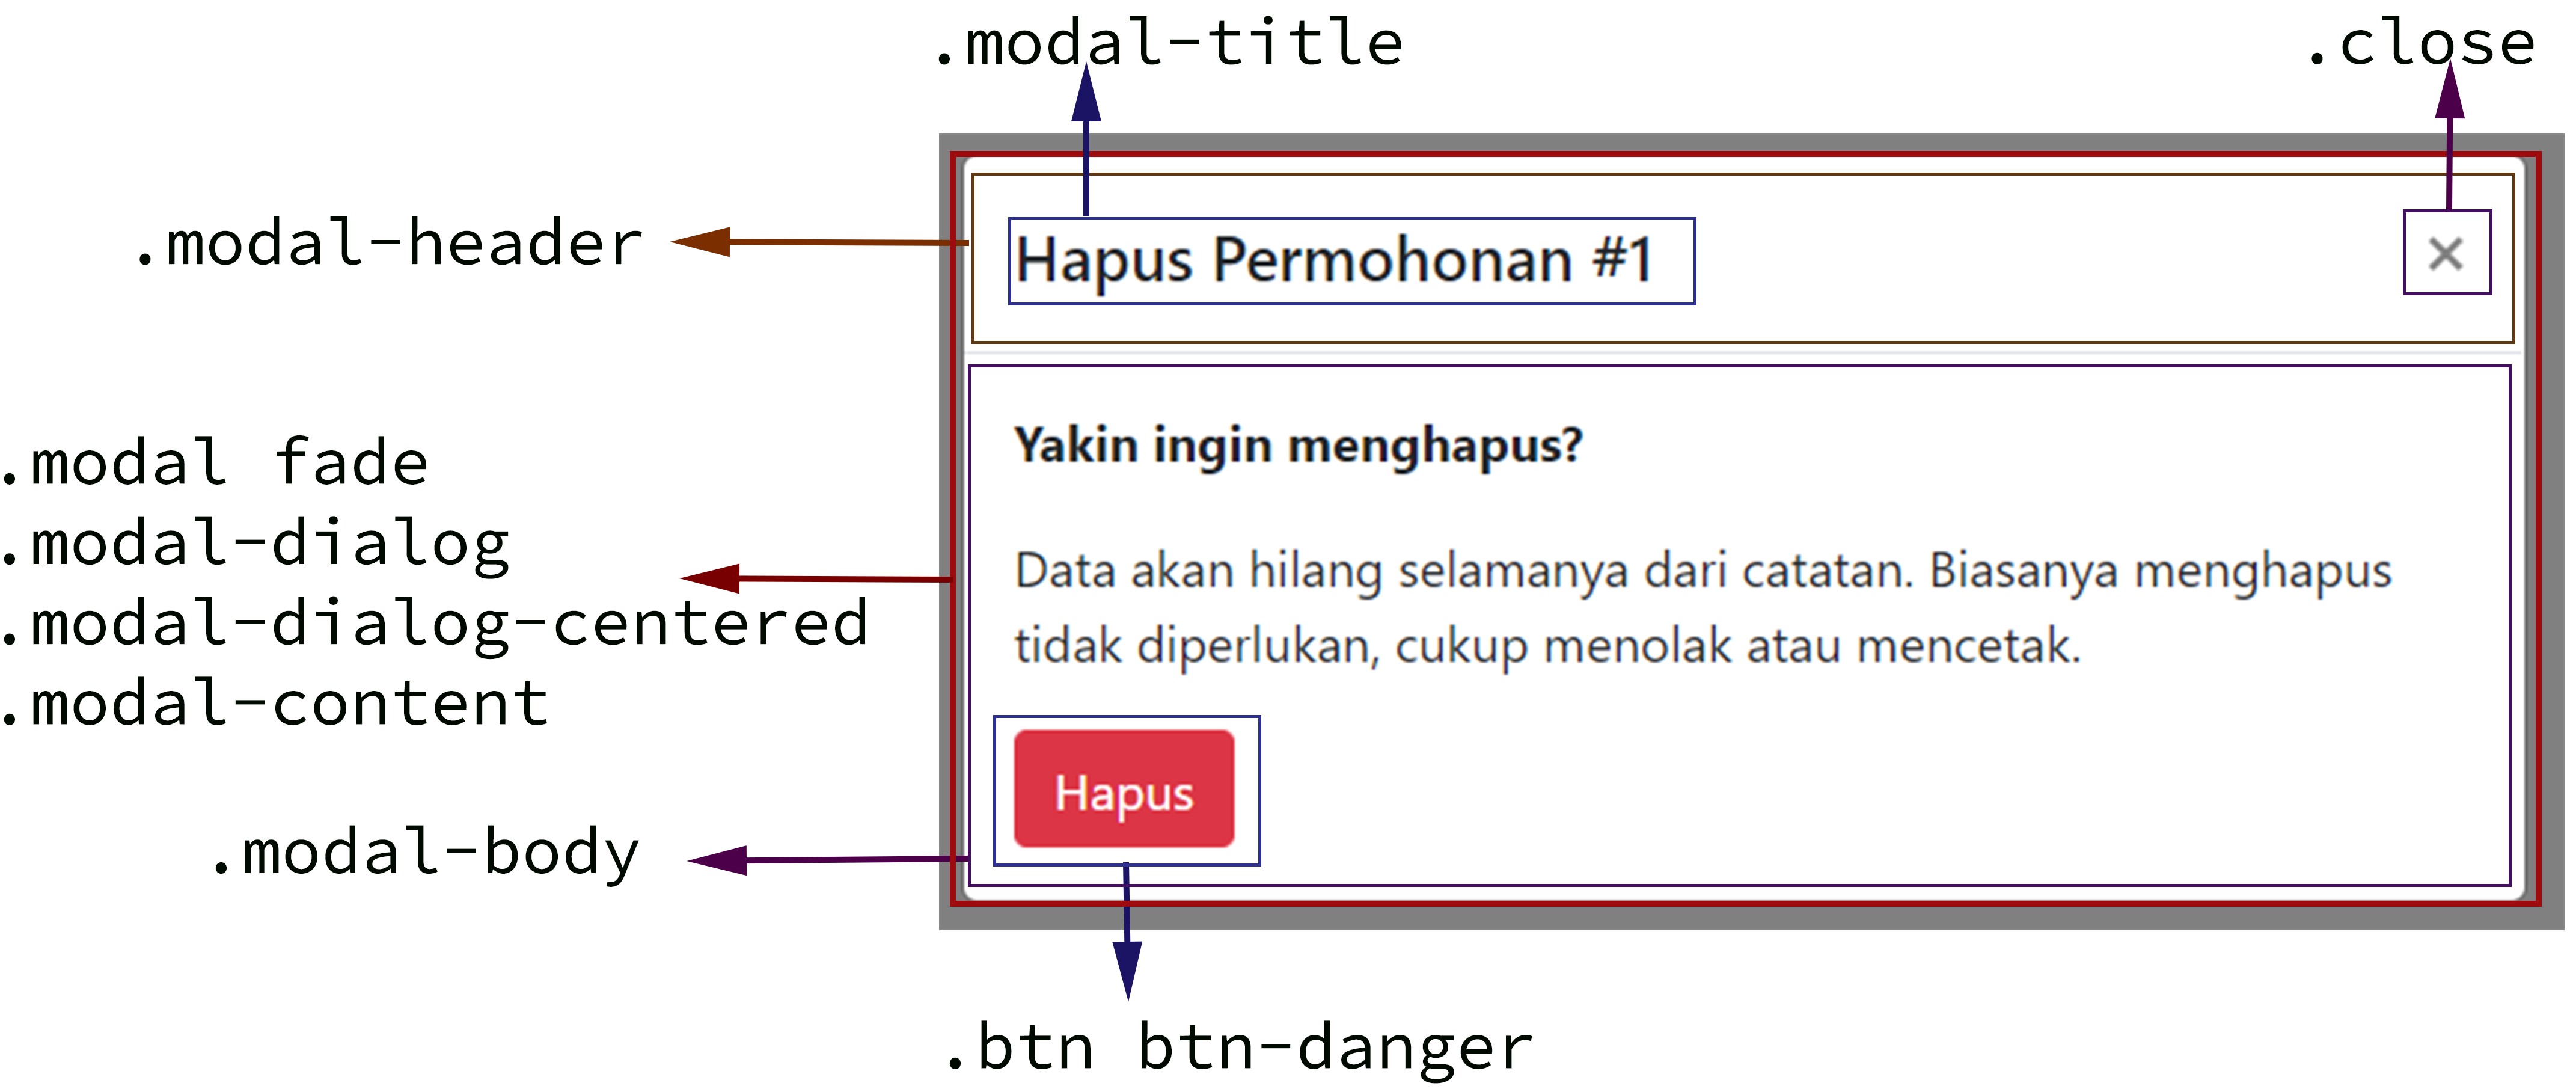
\includegraphics[width=\textwidth,height=\textheight,keepaspectratio]{bootstrap/konversi_modal_trash_manajemen_cetak_transkrip.png}
	\caption{Konversi Modal Hapus} 
\end{figure}
Komponen Modal terdiri dari:
\begin{itemize}
	\item \texttt{.reveal data-reveal}: Membuat modal yang menampung tabel detail permohonan.
	\item \texttt{.close-button data-close aria-label}: Menutup modal yang telah terbuka dengan memberikan label `x' pada tombol.
	\item \texttt{.stack}:	Membuat tabel detail permohonan perubahan kuliah.
\end{itemize}


\subsection{Halaman Perubahan Kuliah}
\subsubsection{Halaman Utama}
\begin{figure} [H]
	\centering  
	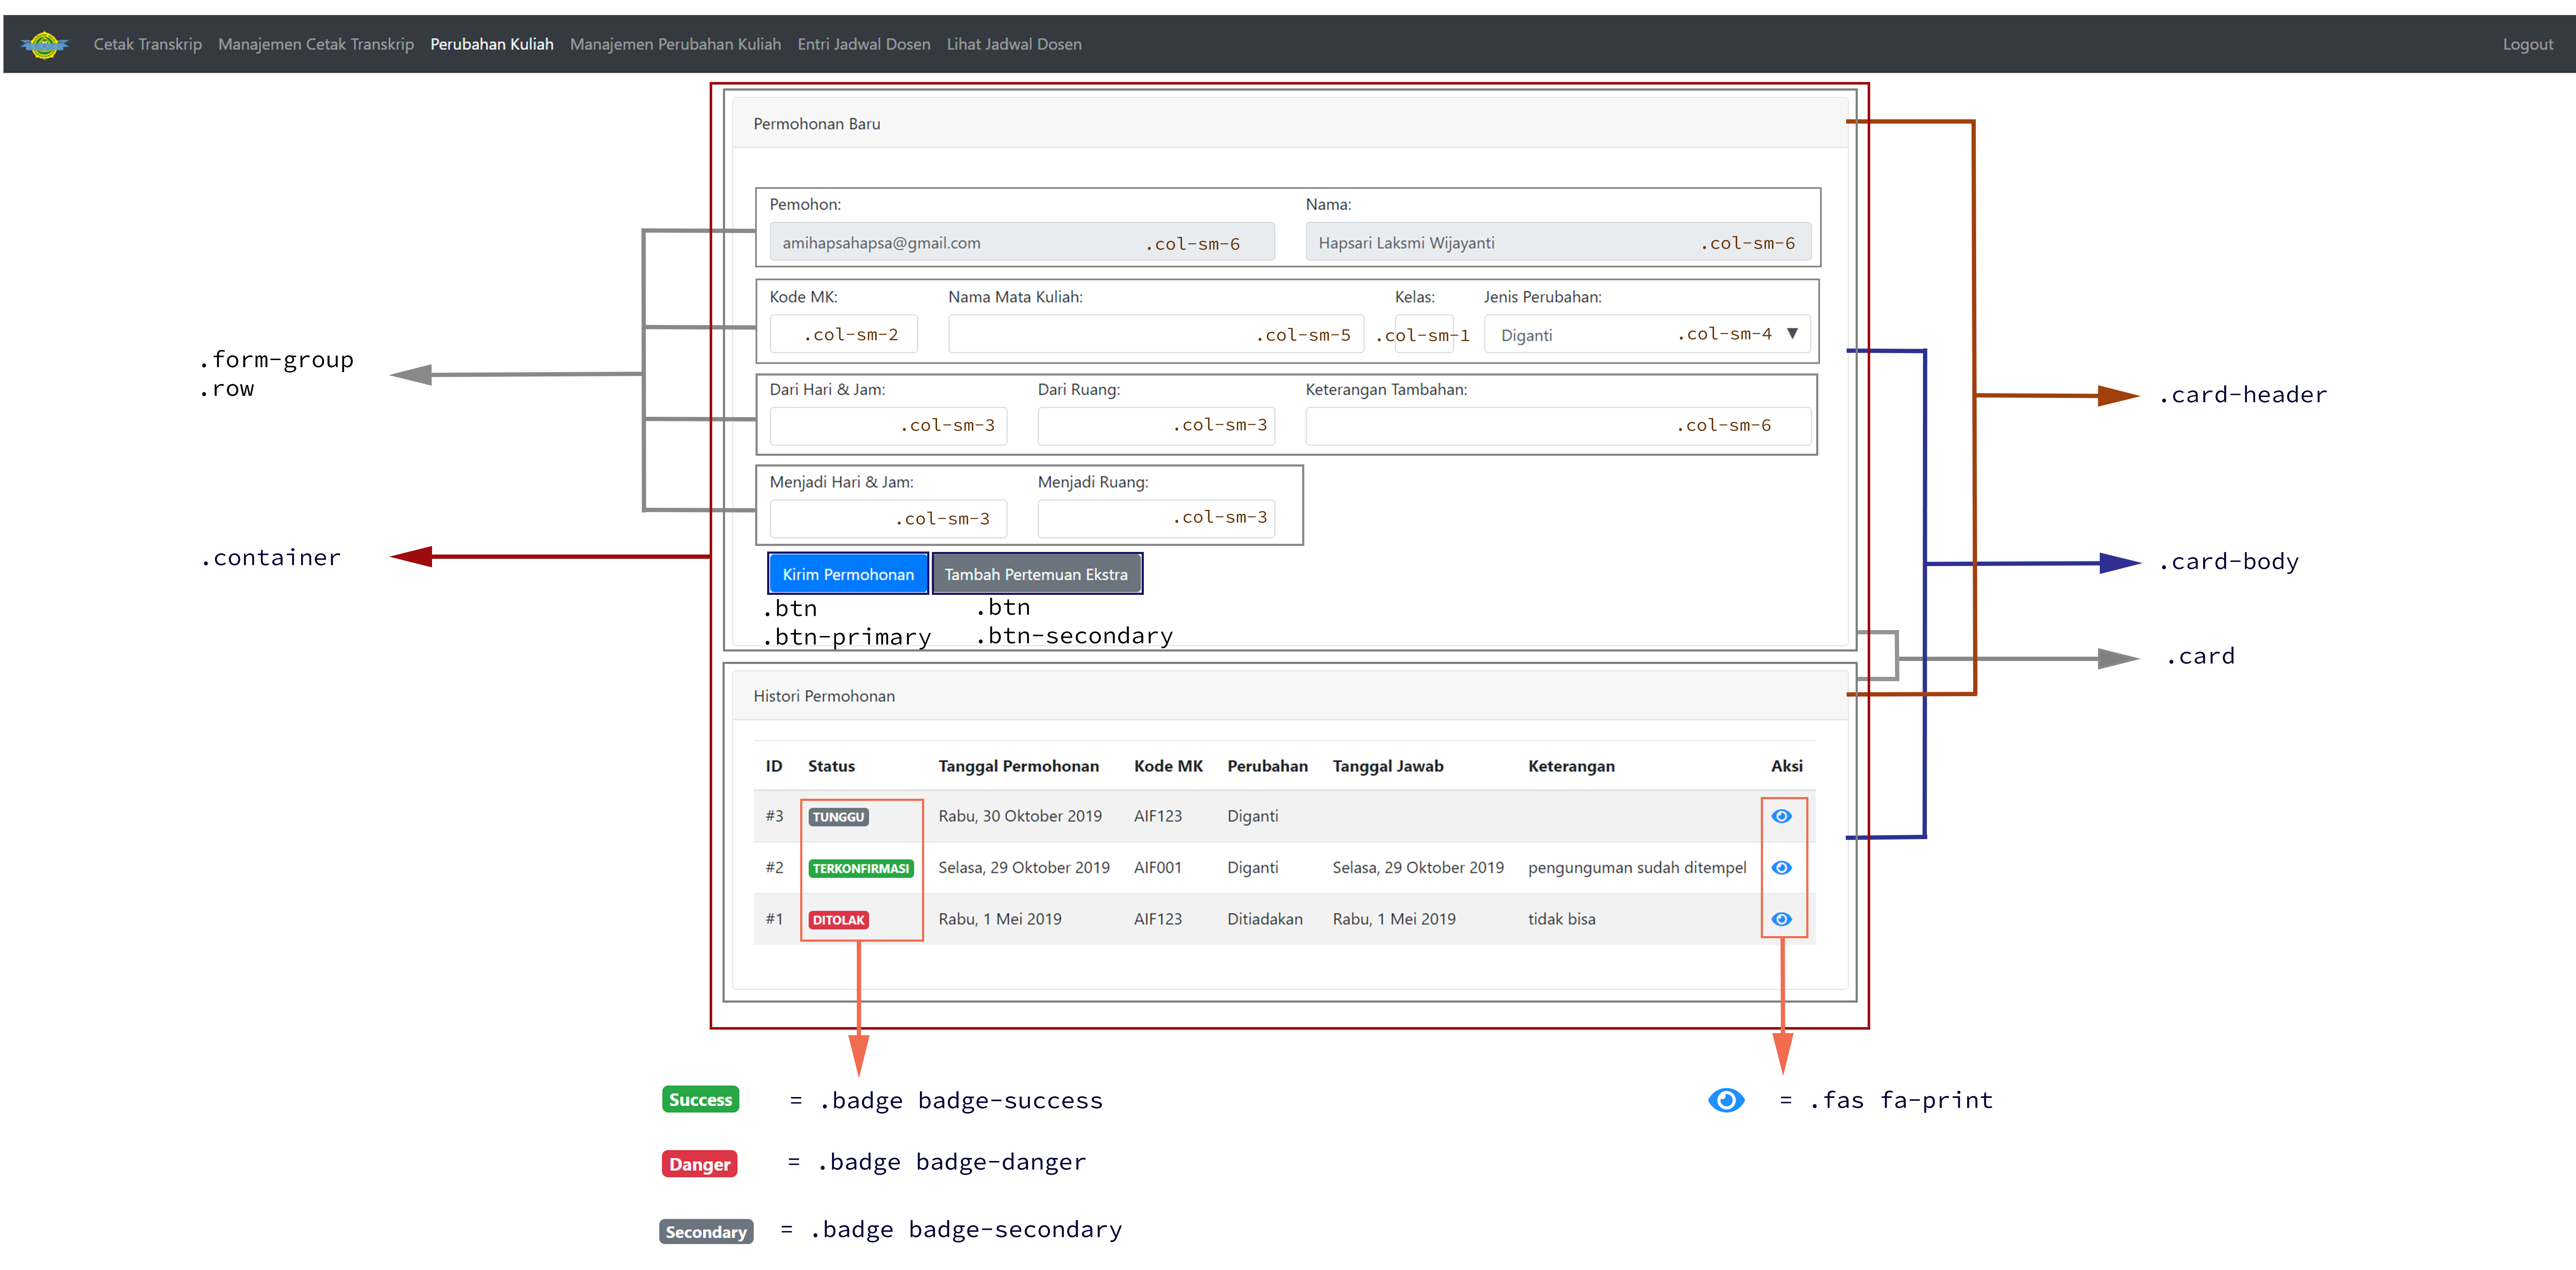
\includegraphics[width=\textwidth,height=\textheight,keepaspectratio]{bootstrap/konversi_tampilan_perubahan_kuliah.png}
	\caption{Konversi Perubahan Kuliah}
\end{figure}
\begin{itemize}
	\item \texttt{.row}: Kelas ini memiliki dua fungsi sebagai container konten dan mengatur beberapa \textit{field-form} menjadi satu baris. 
	\item \texttt{.callout}: Untuk membuat border yang memisahkan konten permohonan baru dan histori permohonan.
	\item \texttt{.stack}: Jenis tabel yang digunakan tabel histori permohonan, sehingga pada layar medium tabel akan tersusun secara bertumpuk.
	\item Ikon Font Awesome yang terdiri dari 
	\begin{itemize}
		\item \texttt{.fas fa-eye data-open}: Ikon untuk menuju modal lihat detail permohonan berdasarkan ID.
	\end{itemize}
	\item Label: Terdiri dari tiga jenis kelas:
	\begin{itemize}
		\item \texttt{.label success}: Label untuk perubahan kuliah berhasil.
		\item \texttt{.label alert}: Label untuk perubahan kuliah gagal.
		\item \texttt{.label warning}: Label untuk perubahan kuliah diproses.
	\end{itemize}
	
\end{itemize}
%Modal: eye
\subsubsection{Modal}
\begin{figure} [H]
	\centering  
	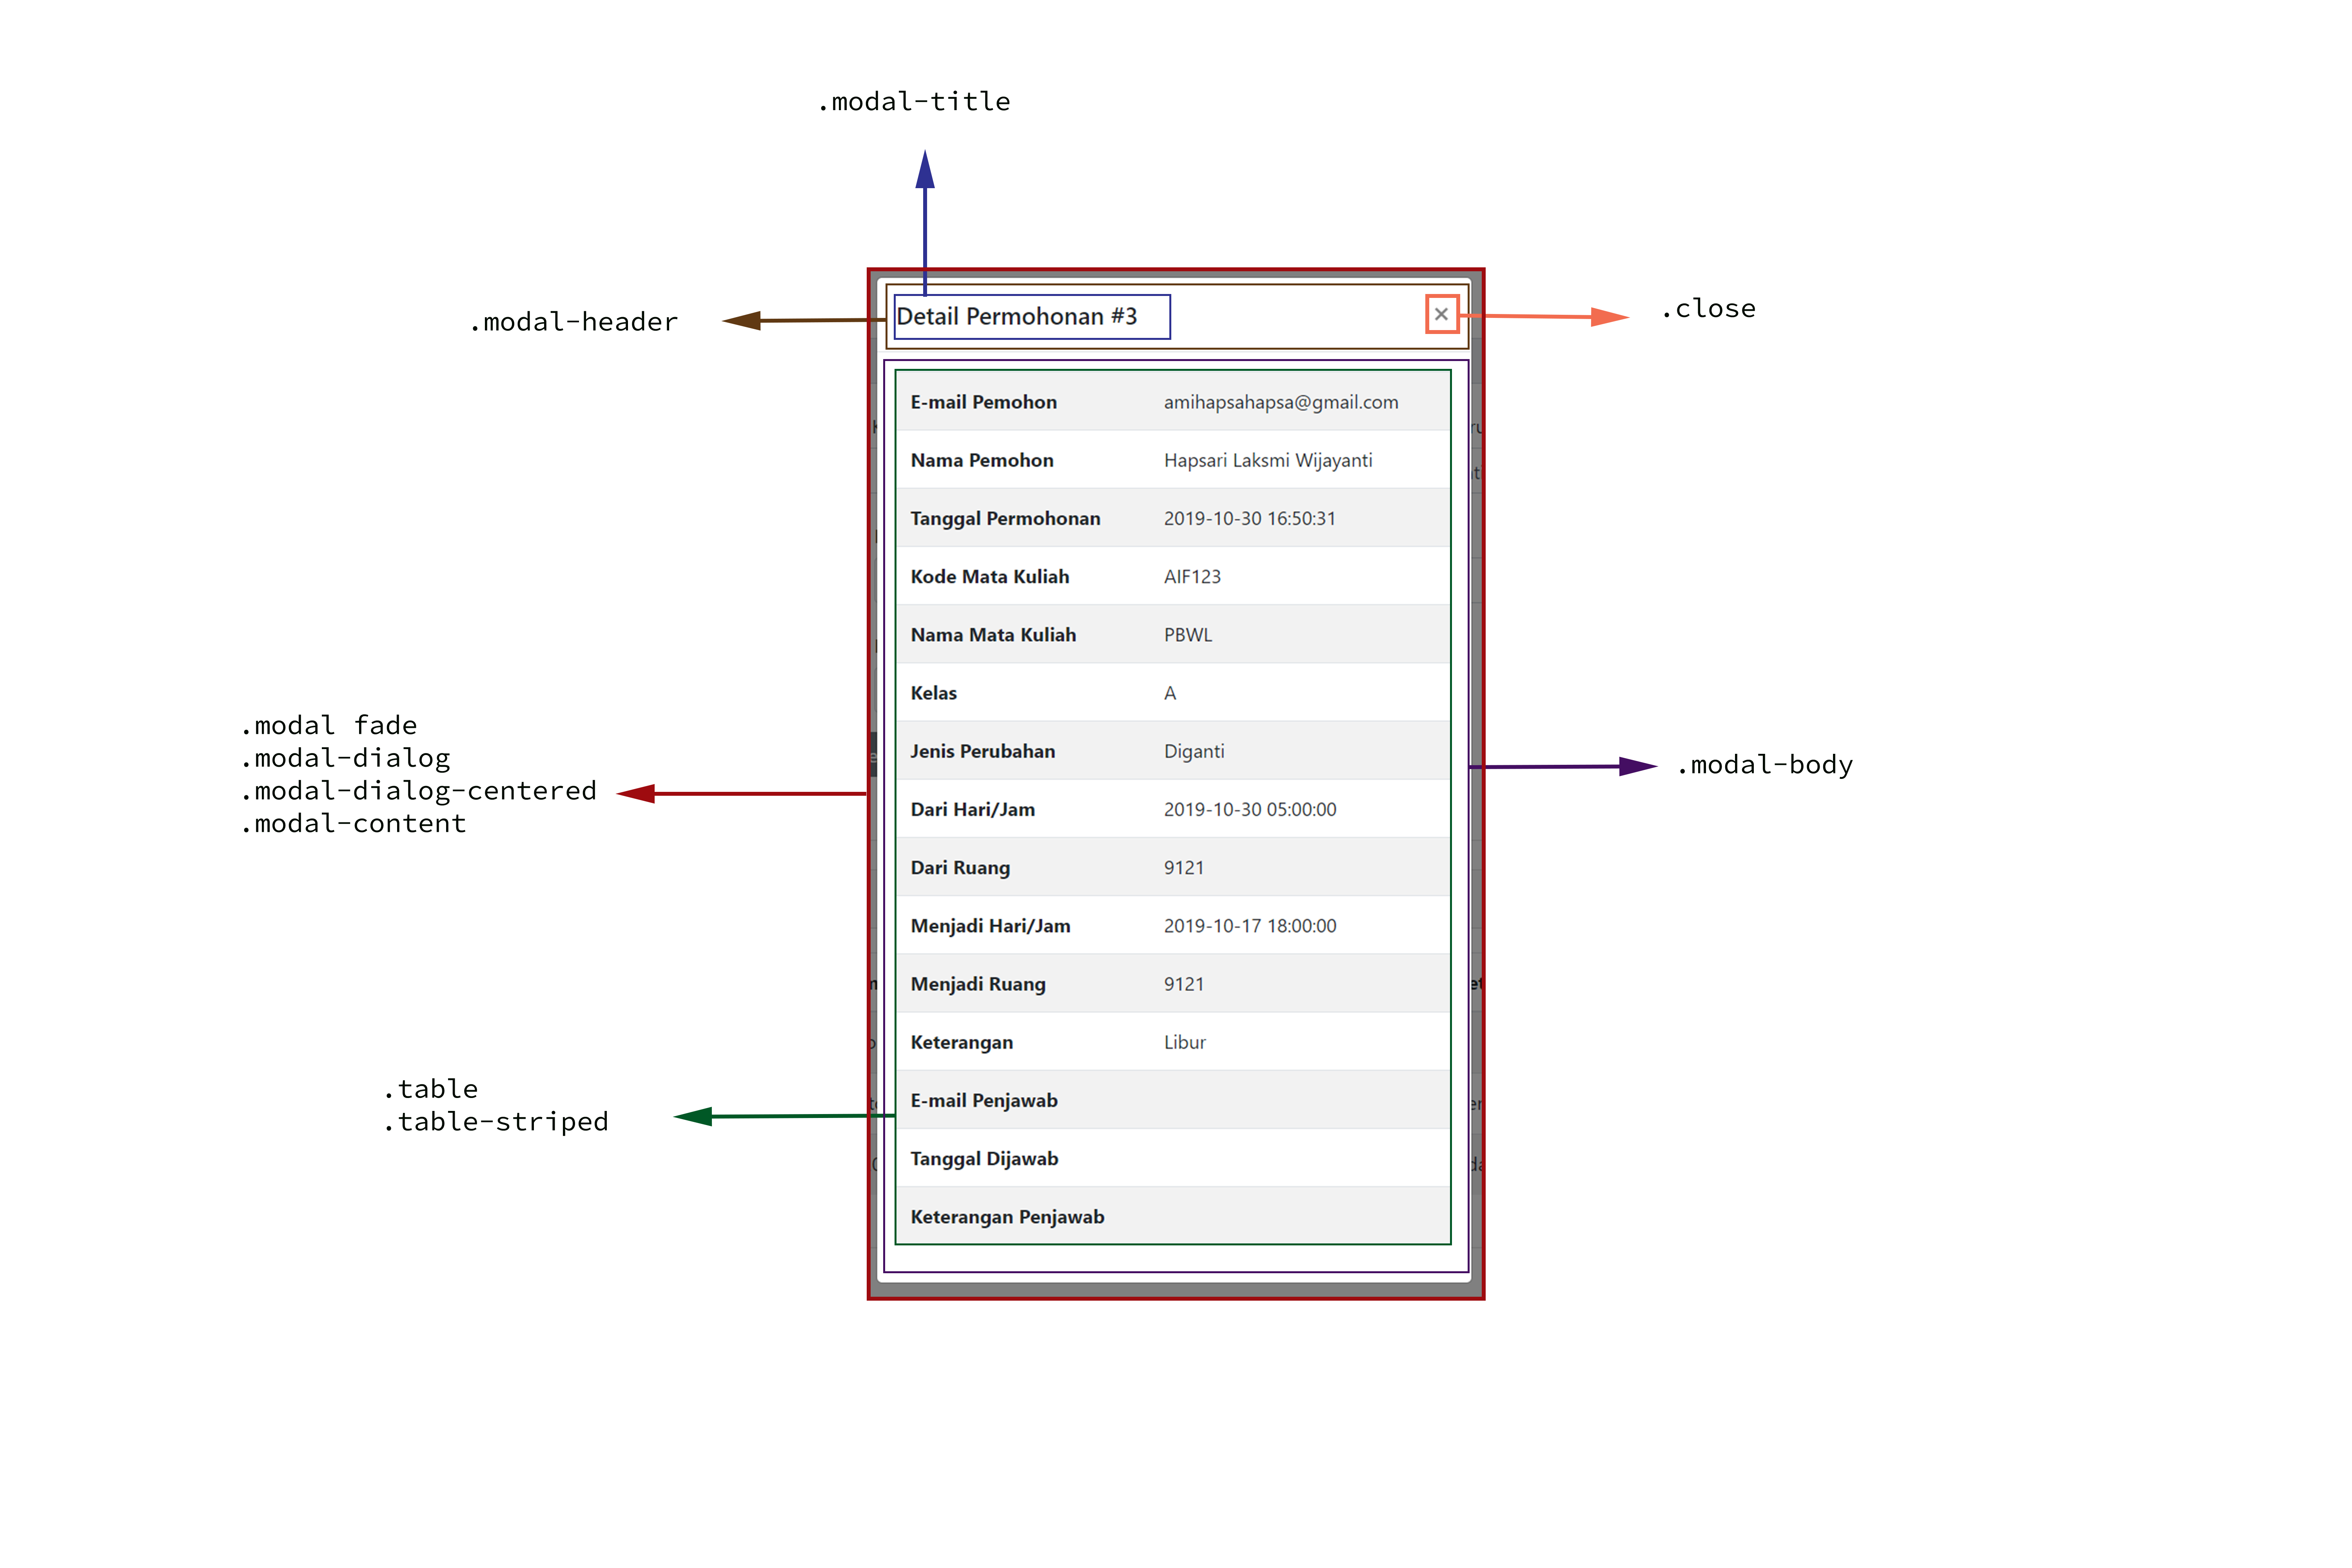
\includegraphics[width=\textwidth,height=\textheight,keepaspectratio]{bootstrap/konversi_modal_lihat_perubahan_kuliah.png}
	\caption{Konversi Modal Lihat}
\end{figure}
Komponen Modal terdiri dari:
\begin{itemize}
	\item \texttt{.reveal data-reveal}: Membuat modal yang menampung tabel detail permohonan.
	\item \texttt{.close-button data-close aria-label}: Menutup modal yang telah terbuka dengan memberikan label `x' pada tombol.
	\item \texttt{.stack}:	Membuat tabel detail permohonan perubahan kuliah.
\end{itemize}


\subsection{Halaman Manajemen Perubahan Kuliah}
\subsubsection{Halaman Utama}
\begin{figure} [H]
	\centering  
	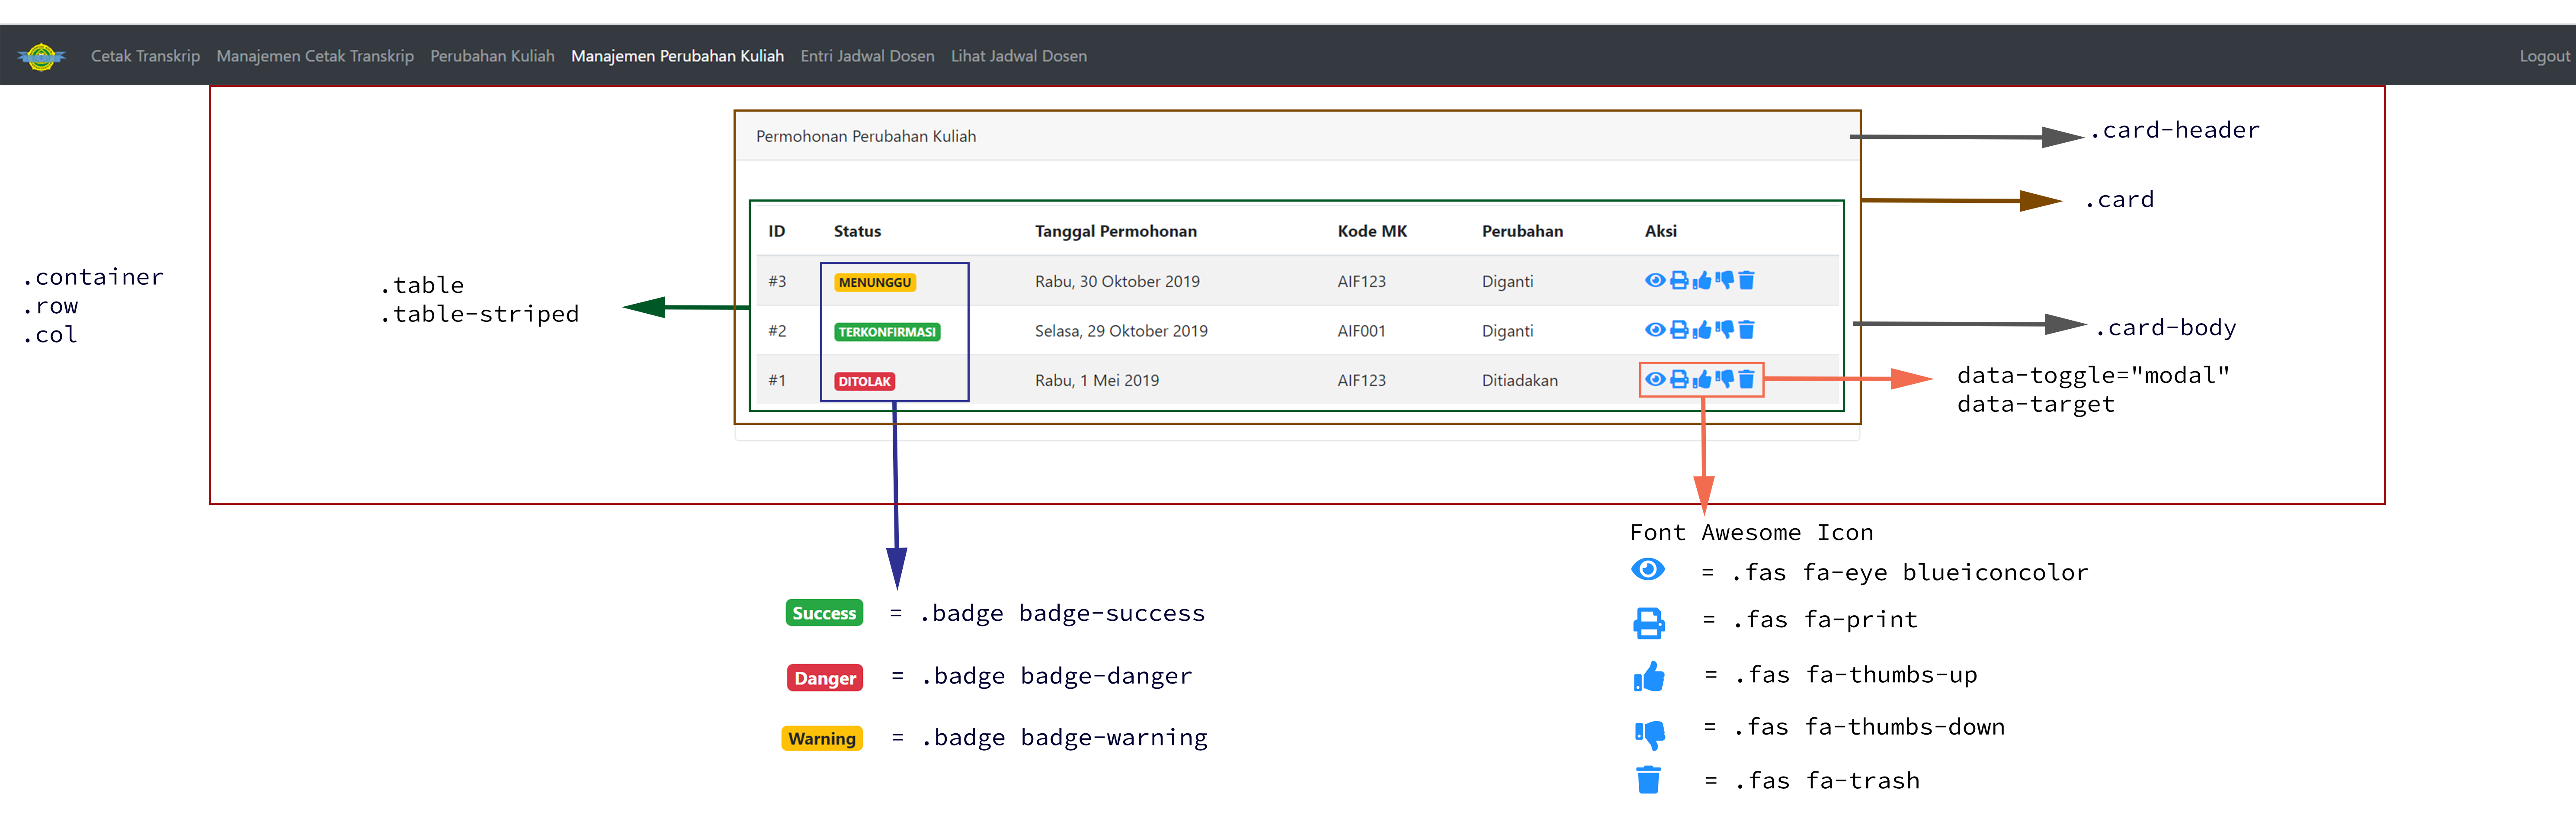
\includegraphics[width=\textwidth,height=\textheight,keepaspectratio]{bootstrap/konversi_tampilan_manajemen_perubahan_kuliah.png}
	\caption{Konversi Halaman Manajemen Perubahan Kuliah}
\end{figure}
\begin{itemize}
	\item \texttt{.row}: Kelas ini memiliki dua fungsi sebagai container konten dan mengatur beberapa \textit{field-form} menjadi satu baris. 
	\item \texttt{.callout}: Untuk membuat border yang memisahkan konten permohonan baru dan histori permohonan.
	\item \texttt{.stack}: Jenis tabel yang digunakan tabel histori permohonan, sehingga pada layar medium tabel akan tersusun secara bertumpuk.
	\item Ikon Font Awesome yang terdiri dari 
	\begin{itemize}
		\item \texttt{.fas fa-eye}: Ikon menuju modal lihat permohonan perubahan kuliah.
		\item \texttt{.fas fa-like}: Ikon menuju modal persetujuan permohonan perubahan kuliah.
		\item \texttt{.fas fa-dislike}: Ikon menuju modal persetujuan penolakan perubahan kuliah.
		\item \texttt{.fas fa-print}: Ikon untuk menuju halaman cetak jadwal perubahan kuliah.
		\item \texttt{.fas fa-trash}: Ikon untuk menghapus permitaan perubahan kuliah.
	\end{itemize}
	\item Label: Terdiri dari tiga jenis kelas:
	\begin{itemize}
		\item \texttt{.label success}: Label untuk permitaan perubahan kuliah telah disetujui.
		\item \texttt{.label alert}:  Label untuk permitaan perubahan kuliah telah ditolak.
		\item \texttt{.label warning}: Label untuk permintaan perubahan kuliah sedang diproses.
	\end{itemize}
	
\end{itemize}
%Modal: lengkap
\subsubsection{Modal}
\begin{figure} [H]
	\centering  
	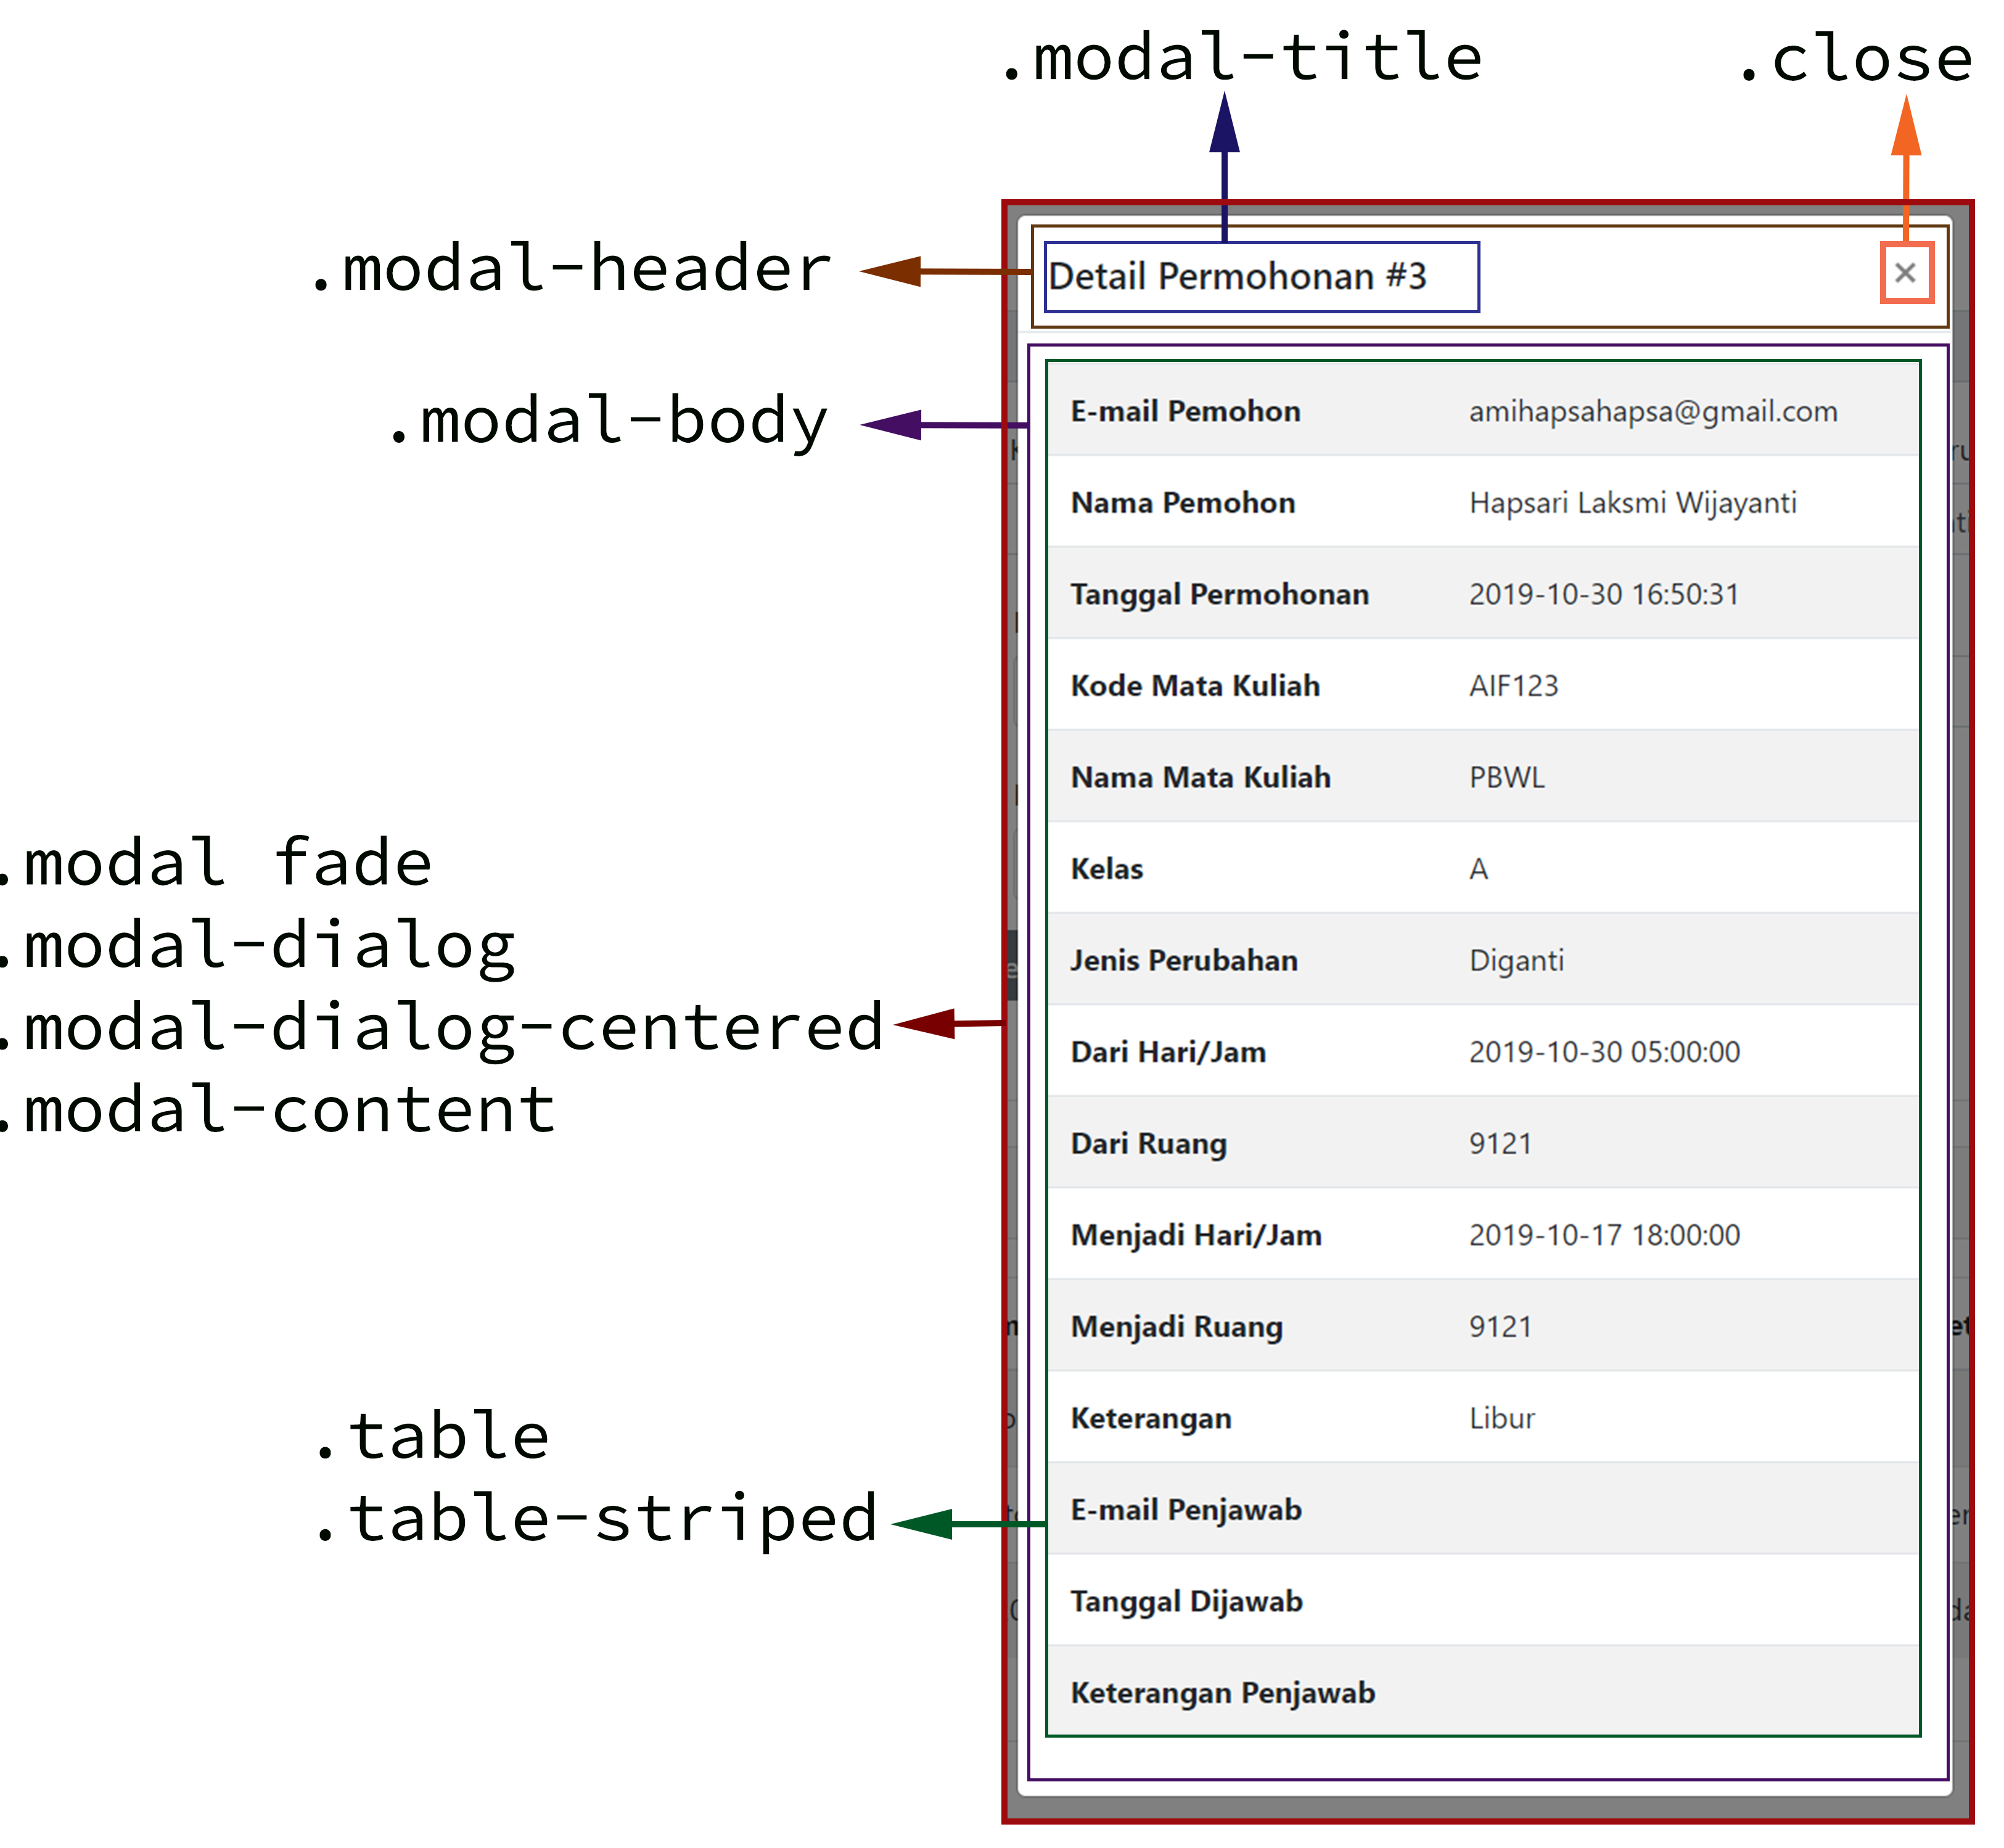
\includegraphics[width=\textwidth,height=\textheight,keepaspectratio]{bootstrap/konversi_modal_lihat_manajemen_perubahan_kuliah.png}
	\caption{Konversi Modal Lihat}
\end{figure}

\begin{figure} [H]
	\centering  
	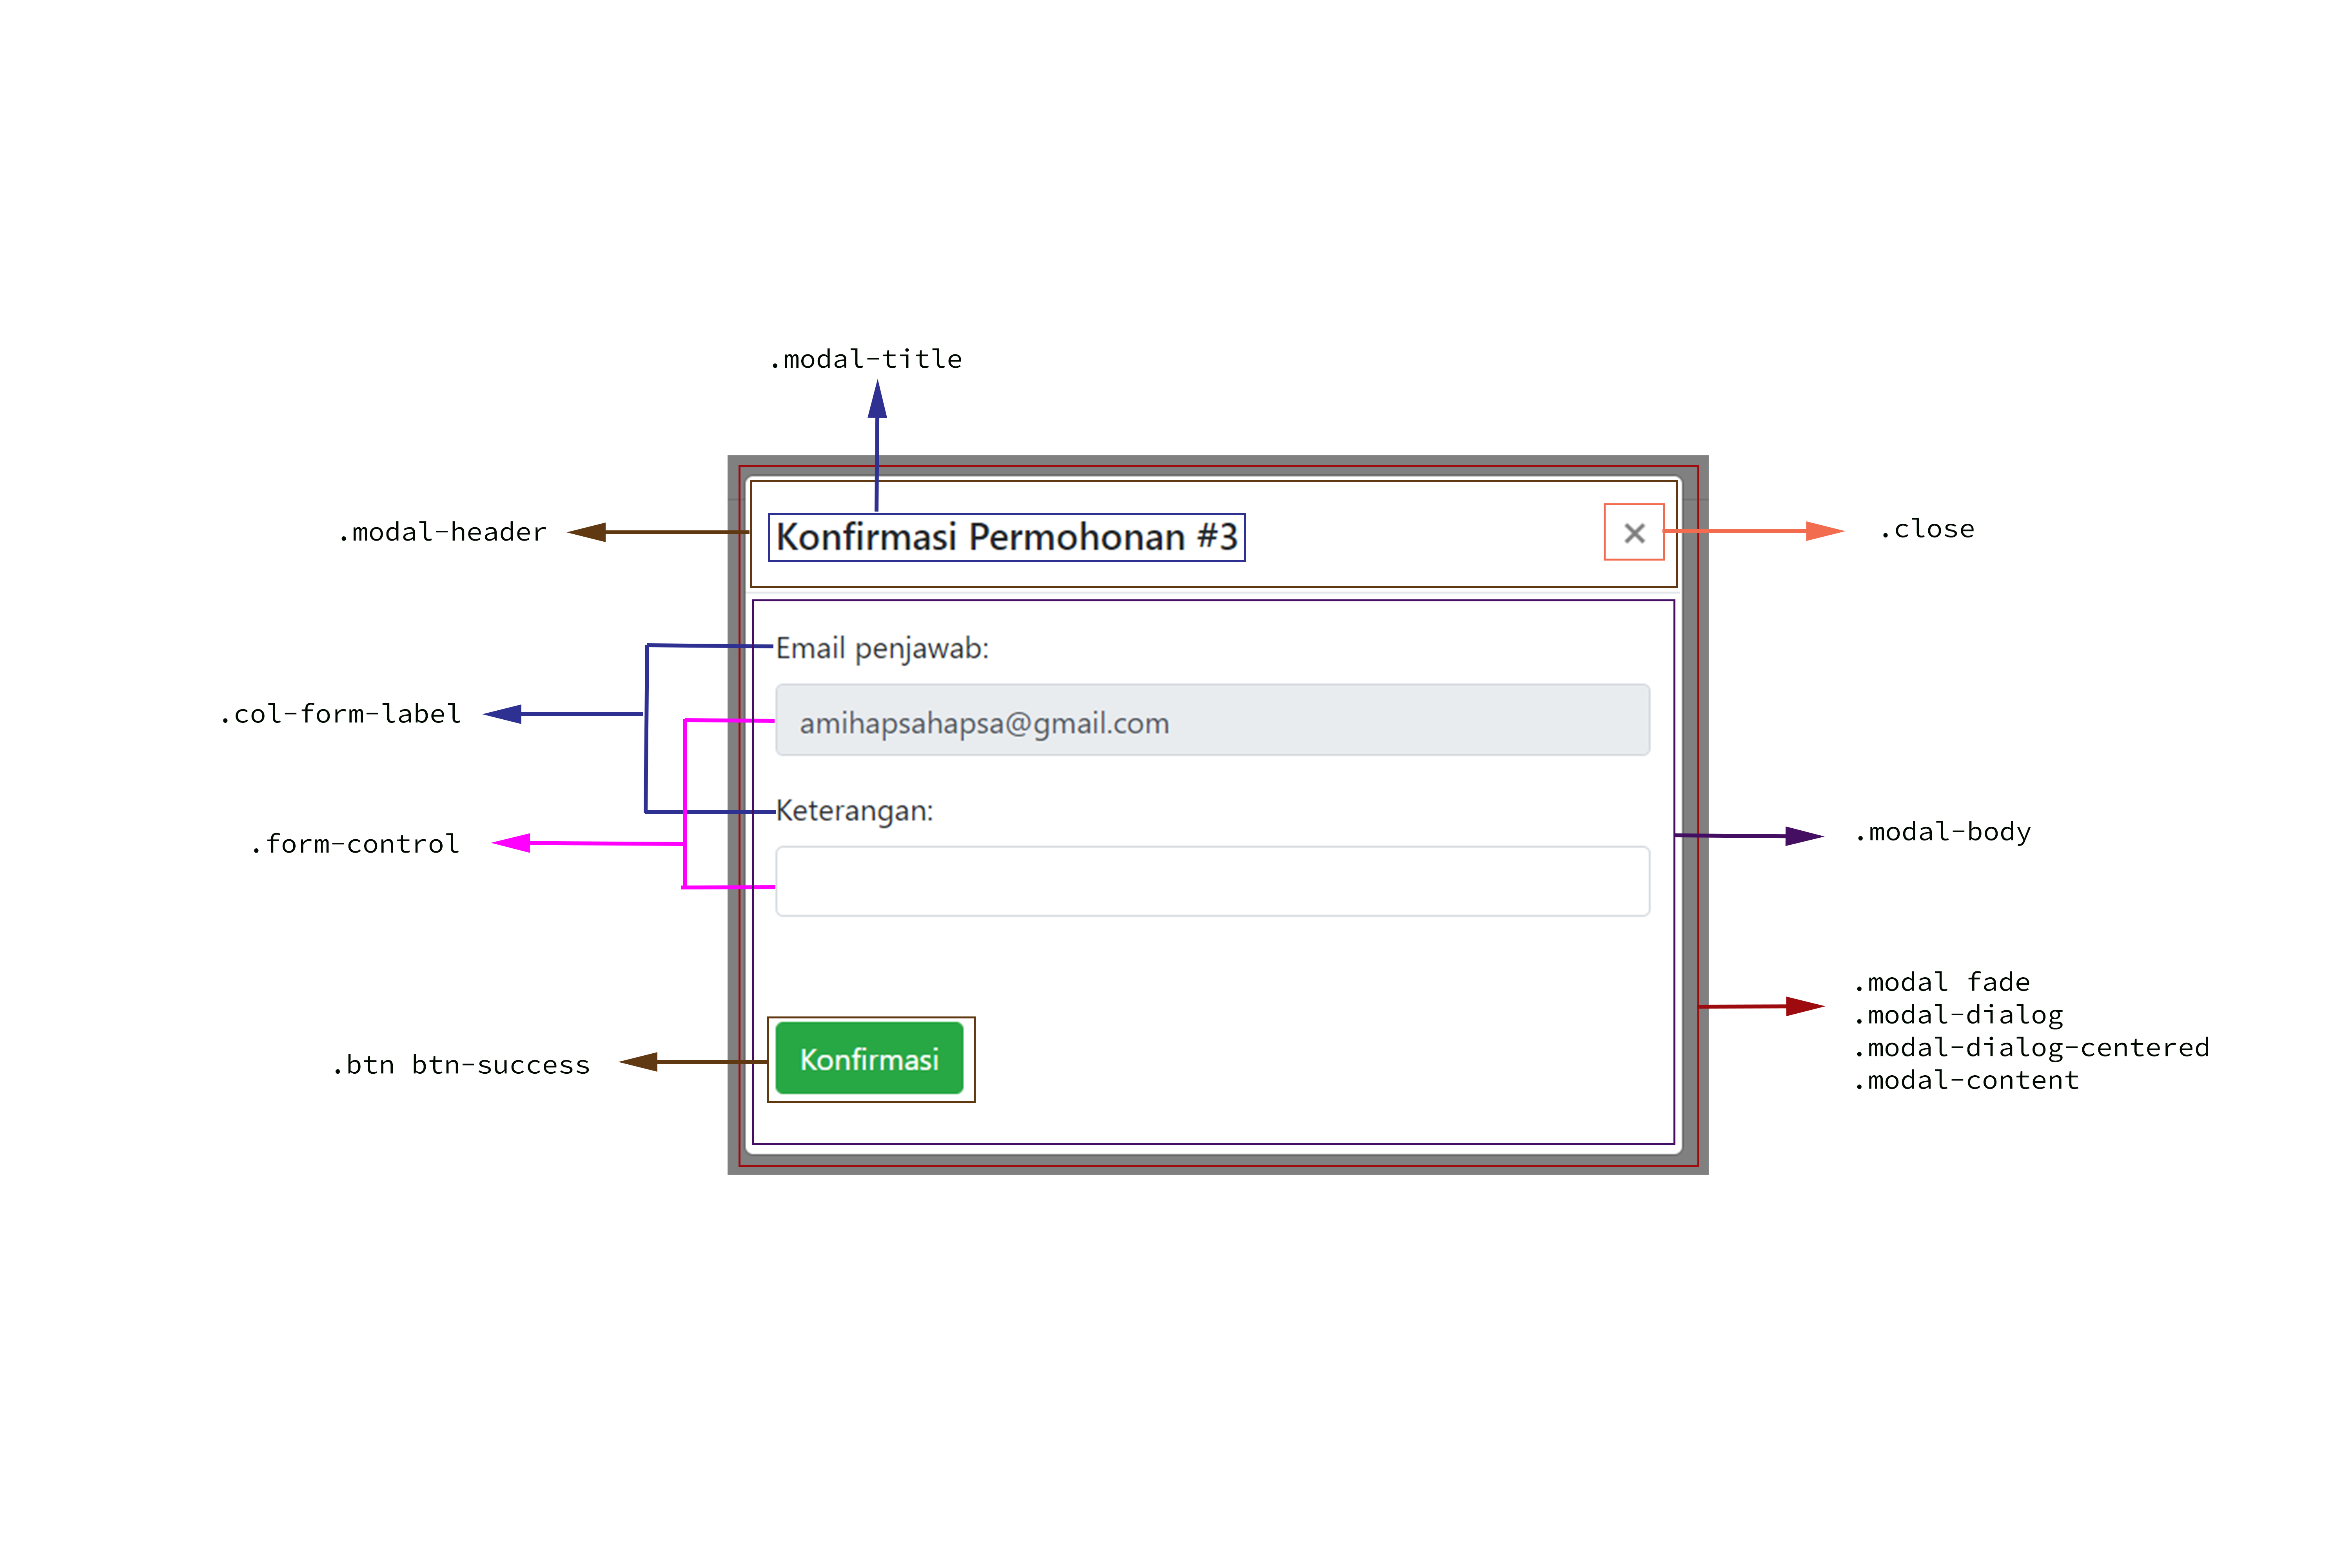
\includegraphics[width=\textwidth,height=\textheight,keepaspectratio]{bootstrap/konversi_modal_like_manajemen_perubahan_kuliah.png}
	\caption{Analisis Modal Setuju}
\end{figure}

\begin{figure} [H]
	\centering  
	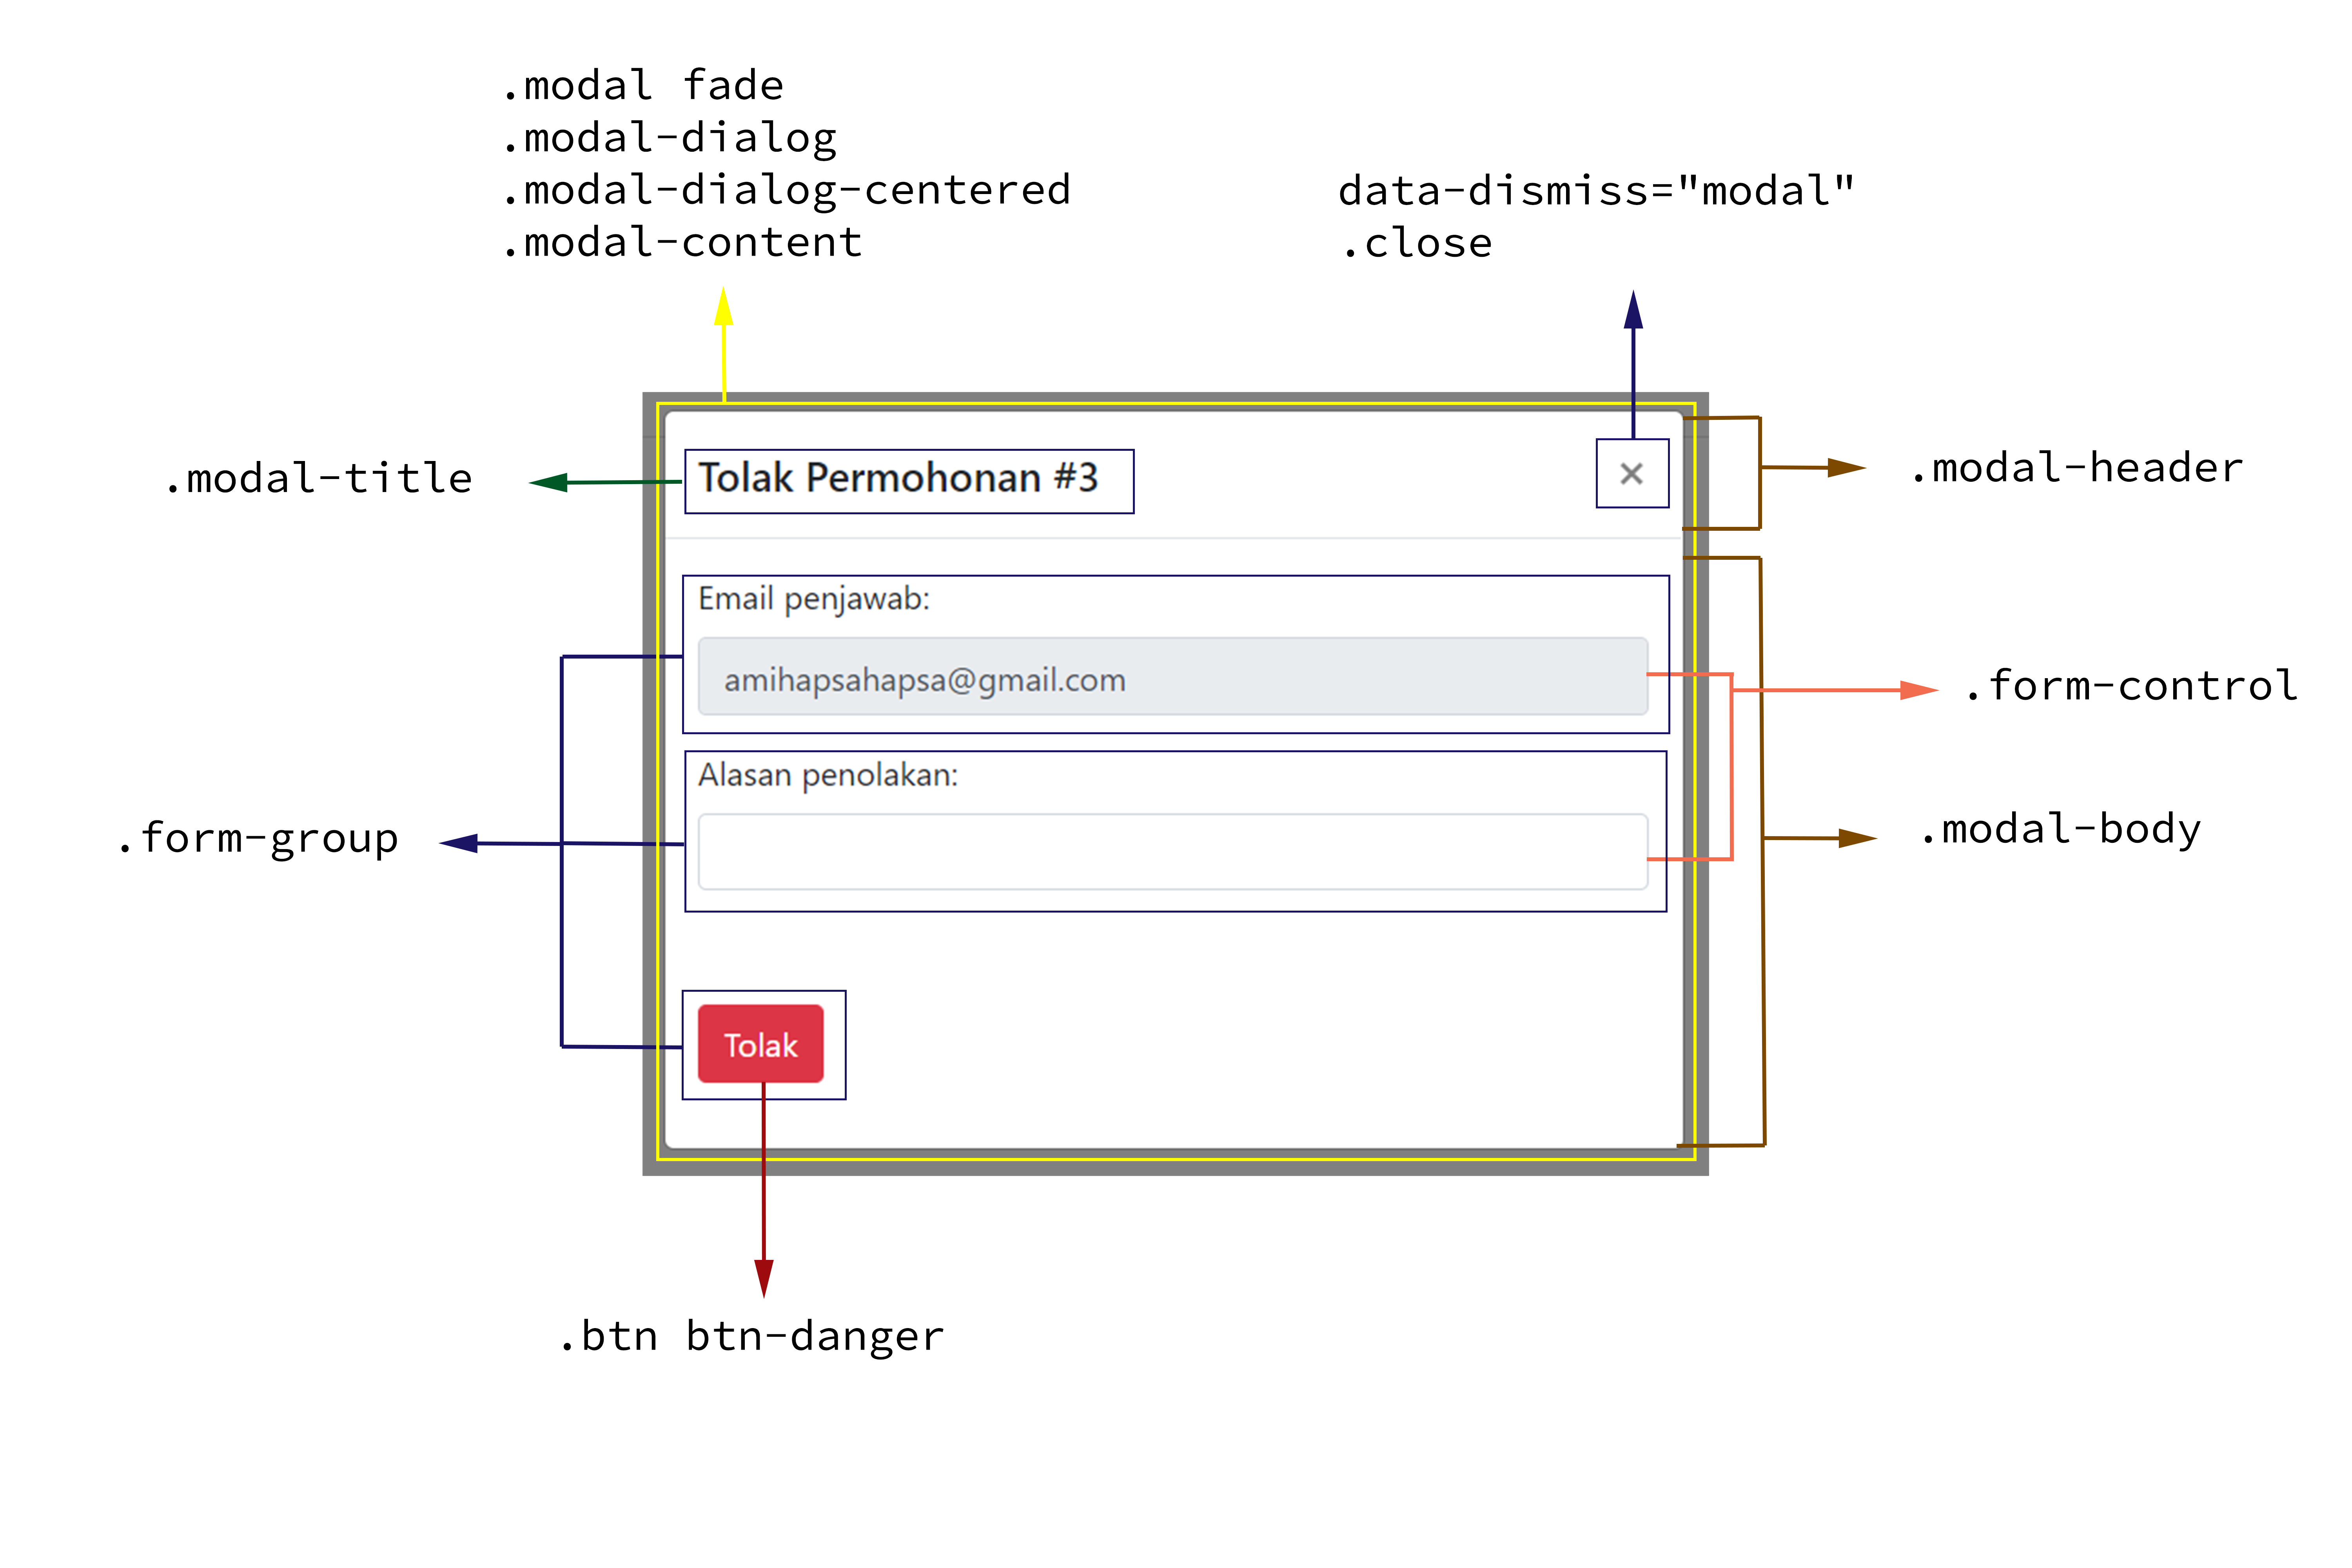
\includegraphics[width=\textwidth,height=\textheight,keepaspectratio]{bootstrap/konversi_modal_dislike_manajemen_perubahan_kuliah.png}
	\caption{Konversi Modal Tolak}
\end{figure}

\begin{figure} [H]
	\centering  
	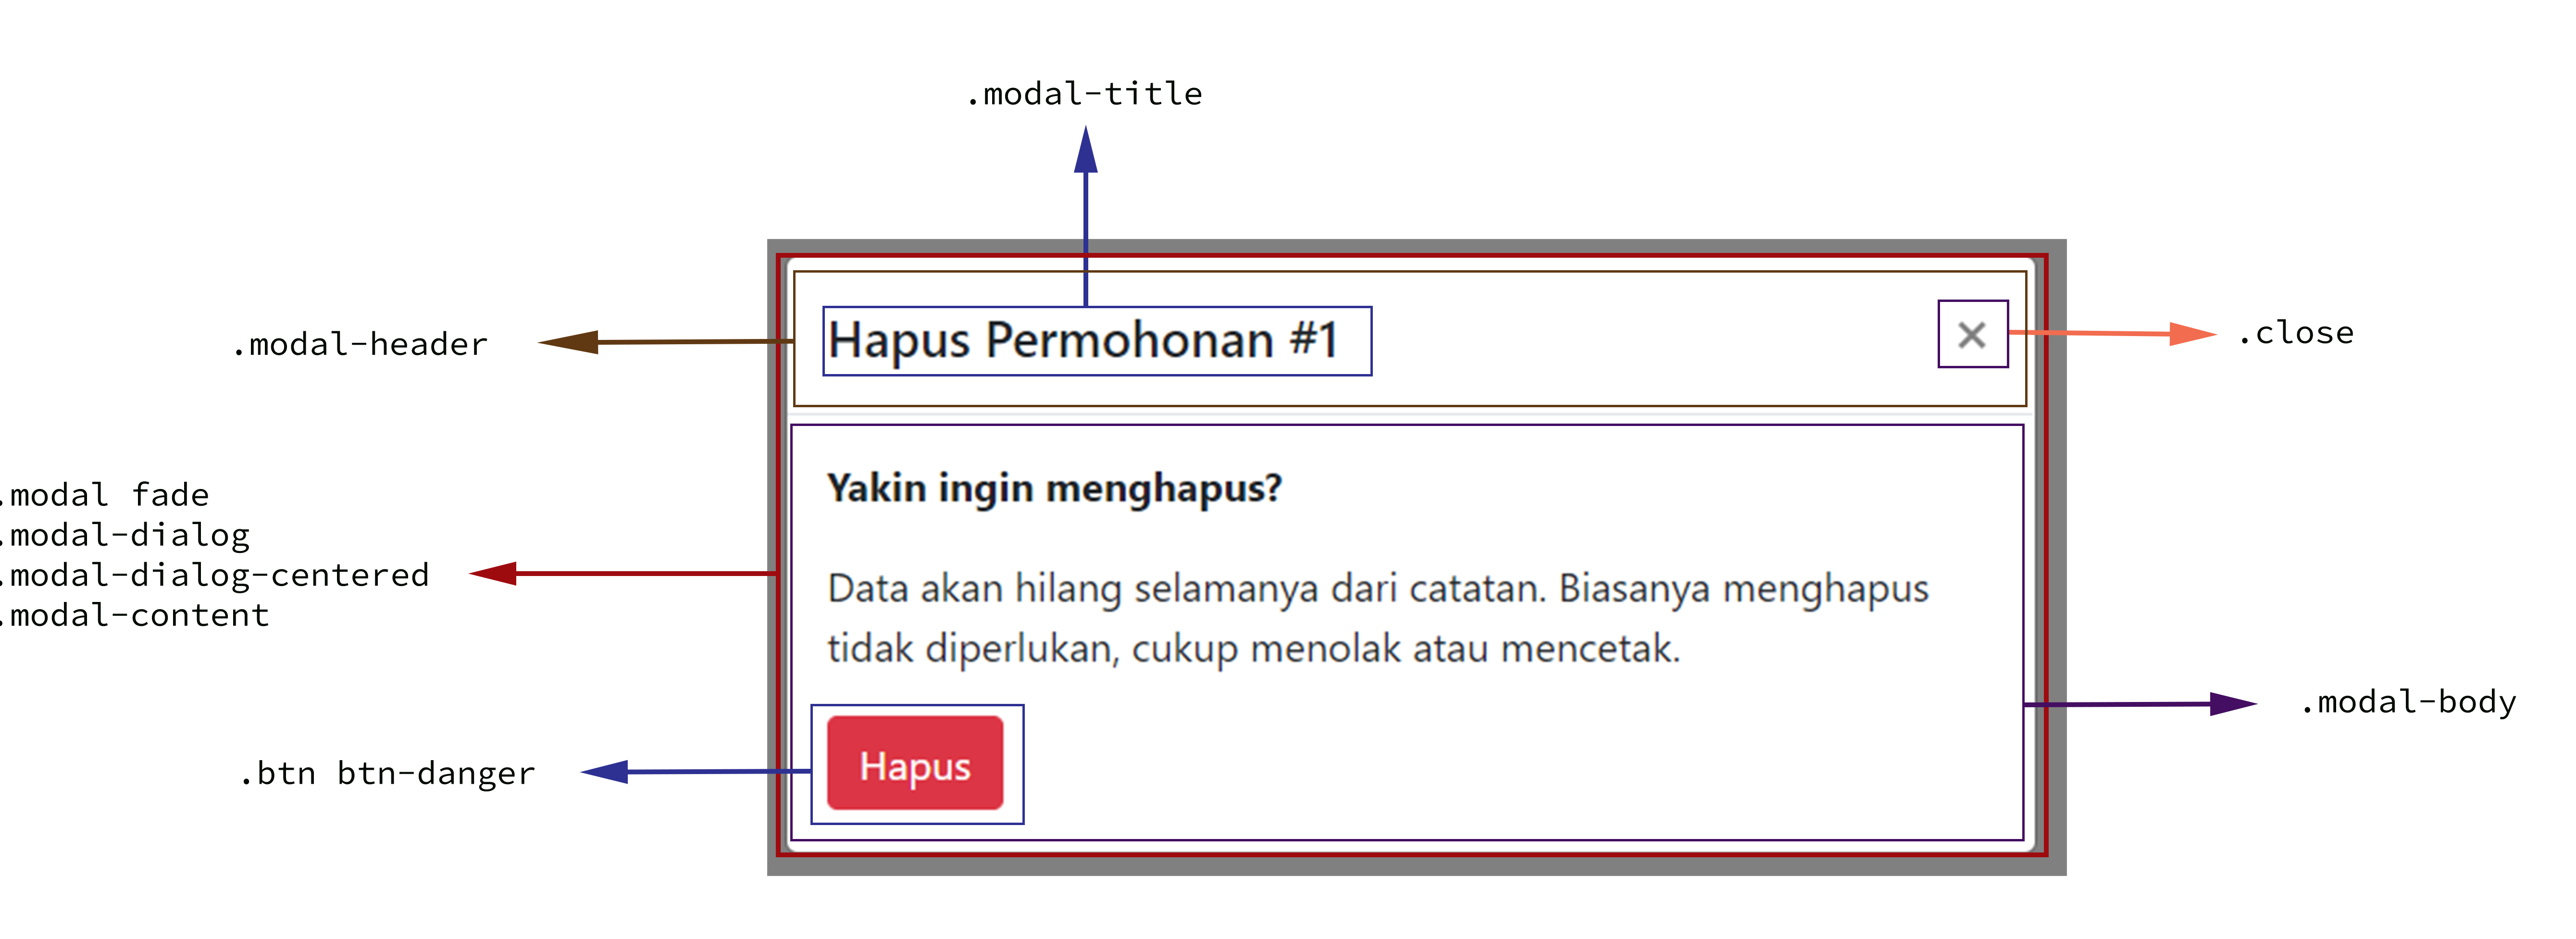
\includegraphics[width=\textwidth,height=\textheight,keepaspectratio]{bootstrap/konversi_modal_trash_manajemen_perubahan_kuliah.png}
	\caption{Konversi Modal Hapus}
\end{figure}
Komponen Modal terdiri dari:
\begin{itemize}
	\item \texttt{.reveal data-reveal}: Membuat modal yang menampung tabel detail permohonan.
	\item \texttt{.close-button data-close aria-label}: Menutup modal yang telah terbuka dengan memberikan label `x' pada tombol.
	\item \texttt{.stack}:	Membuat tabel detail permohonan perubahan kuliah.
	\item \texttt{.alert button}: Membuat button pada tombol `tolak'  dan `hapus'.
\end{itemize}



\subsection{Halaman Entri Jadwal Dosen}
\subsubsection{Halaman Utama}

\begin{figure} [H]
	\centering  
	\includegraphics[width=\textwidth,height=\textheight,keepaspectratio]{bootstrap/konversi_entri_jadwal_dosen.png}
	\caption{Konversi Halaman Entri Jadwal Dosen}
\end{figure}
\begin{itemize}
	\item \texttt{.row}: Kelas ini memiliki dua fungsi sebagai container konten dan mengatur beberapa \textit{field-form} menjadi satu baris. 
	\item \texttt{.large-4 column}: Setiap field akan pada \textit{form} Tambah Jadwal akan memiliki lebar masing-maisng 4 grid pada layar \textit{large}.
	\item \texttt{.large-12 column}: Konten Tambah Jadwal dan Daftar Jadwal memiliki lebar 12 grid.
	\item \texttt{.callout}: Untuk membuat border yang memisahkan konten tambah jadwal dan detail jadwal.
	\item \texttt{.table-scroll}: Membuat tabel daftar jadwal dapat digerakan secara horizontal.
	\item \texttt{button}: Membuat button pada tombol `Ekspor ke XLS' untuk konten Daftar Jadwal dan `Tambah' pada konten Tambah Jadwal.
	\item \texttt{.alert button}: Membuat button pada tombol `Delete All'.
	
\end{itemize}
%Modal: edit
\subsubsection{Edit Jadwal}
-

\subsection{Halaman Lihat Jadwal Dosen}

\begin{figure} [H]
	\centering  
	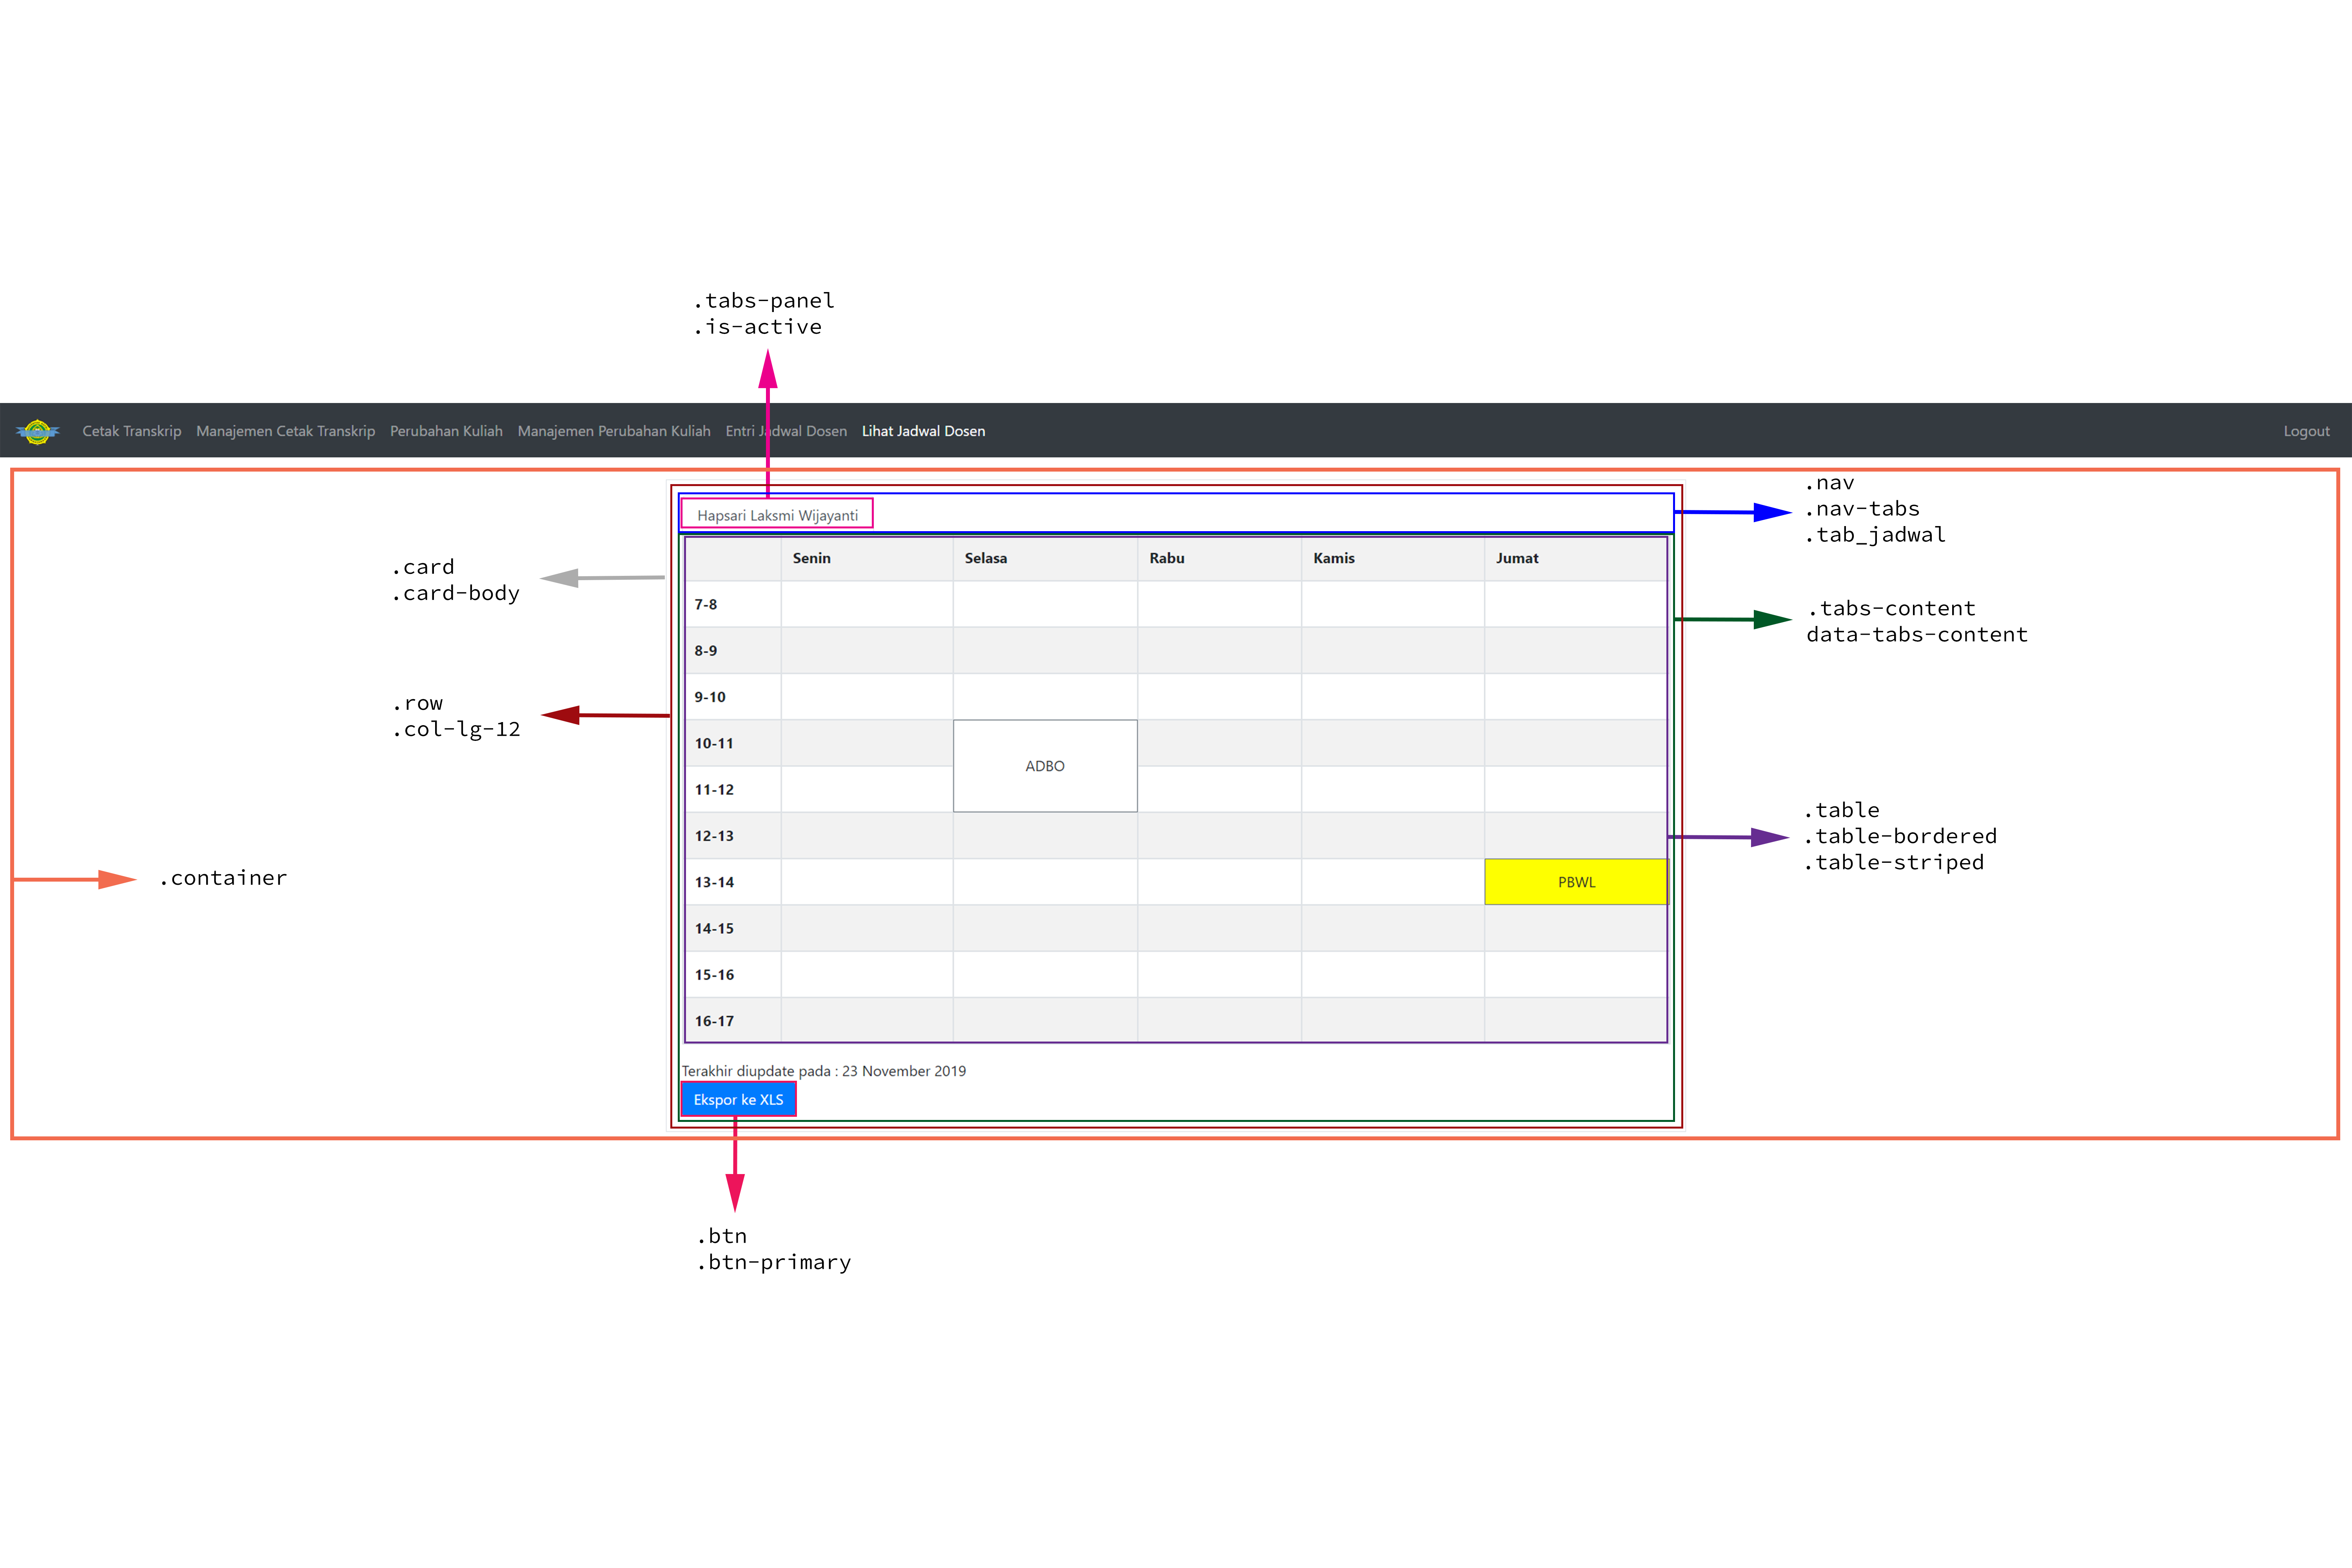
\includegraphics[width=\textwidth,height=\textheight,keepaspectratio]{bootstrap/konversi_lihat_jadwal_dosen.png}
	\caption{Analisis Modal Edit Jadwal}
\end{figure}

\begin{itemize}
	\item \texttt{.row}: Kelas ini memiliki dua fungsi sebagai container konten dan mengatur beberapa \textit{field-form} menjadi satu baris. .
	\item \texttt{.large-12 column}: Konten Tambah Jadwal dan Daftar Jadwal memiliki lebar 12 grid.
	\item \texttt{.callout}: Untuk membuat border yang memisahkan konten tambah jadwal dan detail jadwal.
	\item \texttt{.table-scroll}: Membuat tabel lihat jadwal dapat digerakan secara horizontal.
	\item \texttt{button}: Membuat button pada tombol `Ekspor ke XLS' untuk konten Daftar Jadwal dan `Tambah' pada konten Tambah Jadwal.	
	\item \texttt{.tabs data-tabs}: Kontainer untuk simpan nama dosen
	\item \texttt{.tabs-content data-tabs-content}: Kontainer untuk simpan isi konten dari tabs.
	\item \texttt{.tabs-title}: Kelas untuk judul tabs nama dosen.
	\item \texttt{.is-active}: Menujukkan tabs nama dosen yang sedang dilihat
\end{itemize}








